\section{Prioritised-Timed Coloured Petri Nets}\label{petrinet}

Next, we introduce the specific model of prioritised-timed
coloured Petri net considered for the translation. We use prioritised-timed coloured Petri nets, 
which are
a prioritised-timed extension of coloured Petri nets,
the well-known formalism supported by CPNTools \cite{CPNTools}. In Definition \ref{cpn}, we recall the formal definition of coloured Petri nets presented in \cite{Jensen2009}, whereas, in Definition \ref{ptcpn}, we define the precise model used in this work.
%In this model, places have an associated colour set (data types). 
%Each token then  has  an attached data value
%({\em token colour}),
%which belongs to the colour to which the token is
%associated.

\begin{definition}\label{cpn}
A timed non-hierarchical Coloured Petri Net is a nine-tuple $\it{CPN_{T}}$ = (P, T, A, $\Sigma$ ,V,C, G, E, I) where:
\begin{spacing}{0}
\begin{itemize}
\item P is a finite set of places.
\item T is a finite set of transitions such that $P \cap T = \emptyset$.
\item $A \subseteq (P \times T)\;\cup\;(T \times P)$ is a set of directed arcs.
\item $\Sigma$ is a finite set of non-empty colour sets. Each colour set is either untimed or
timed.
\item V is a finite set of typed variables such that $\textit{Type[v]} \in \Sigma$ for all variables $v \in V$.
\item $C : P \rightarrow \Sigma$ is a colour set function that assigns a colour set to each place. A place
p is timed if C(p) is timed, otherwise p is untimed.
\item $G : T \rightarrow EXPR_V$ is a guard function that assigns a guard to each transition t such
that Type[G(t)] = Bool.
\item $E : A \rightarrow EXPR_V$ is an arc expression function that assigns an arc expression to
each arc a such that
\begin{itemize}
\item \mbox{${\it Type[E(a)] = C(p)_{MS}}$} if p is untimed;
\item \mbox{${\it Type[E(a)] = C(p)_{TMS}}$} if p is timed.
\end{itemize}
Here, p is the place connected to the arc a. Moreover, {\it MS} and {\it TMS} are untimed and timed colour sets in $\Sigma$, respectively.
\item $I : P \rightarrow EXPR_{\emptyset}$ is an initialisation function that assigns an initialisation expression to each place p such that
\begin{itemize}
\item \mbox{${\it Type[I(p)] = C(p)_{MS}}$} if p is untimed;
\item \mbox{${\it Type[I(p)] = C(p)_{TMS}}$} if p is timed.
\end{itemize}
\end{itemize}
\end{spacing}
\vspace{-0.2cm}
\end{definition}

{\flushright $\Box$\\
\mbox{}\vspace{-2ex}}

In this work, we consider a class of $CPN_T$, where three functions have been added. First, a {\em labelling}
function is used to label places and transitions. Transitions can be labelled with either strings
or nothing.  Places are labelled as
{\em entry places}, {\em output places}, {\em error places}, {\em exit places}, 
{\em internal places}, {\em variable places} and
{\em resource places},
which, respectively, correspond to the following labels:
$\{{\it in, ok, er, ex, i, v, r}\}$.  Second, a {\em delay} function to assign a time interval to some transitions. This time interval is uniformly distributed. This is a shorthand for adding this time delay inscription to the time
delay inscription of each output arc expression. Finally, the {\em priority} function assigns priorities to transitions, considering only two levels ${\it P_{LOW}}$ and ${\it P_{NORMAL} (\textmd{by default})}$. 


\begin{definition}\label{ptcpn}%(Prioritised-Timed Coloured Petri Nets)\\
We define a prioritised-timed coloured Petri net (PTCPN)
as a tuple $(CPN_T,\lambda,D,\pi)$, where\footnote{
We use the classical notation on Petri nets to denote the
precondition and postcondition of both places and transitions:
%
\[ \forall x \in P\,\cup\,T\,:\,
\precond{x} = \{ y \,|\, (y,x) \in A\}~~~~~
   x^{\bullet} = \{ y \,|\, (x,y) \in A\}
\]
}:
%
\begin{itemize}
%\item $P$ is a finite set of {\em coloured places}.
%Colours used in this semantics will be introduced progressively,
%as we define the PTCPNs corresponding to each activity. 
%We will use timed and untimed coloured tokens, so timed tokens will 
%have associated a time stamp, according to the CPNTools
%interpretation~\cite{Jensen2009}. 
%%
%\item $T$ is a finite set of {\em transitions} ($P\cap T = \emptyset$).
%%
%\item $A \subseteq (P\times T)\,\cup\,(T \times P)$ is a
%set of directed {\em arcs}.
%%
%%
%\item $V$ is a finite set of {\em integer variables}
%i.e. ${\it Type}(v) \in \entero$, for all $v \in V$.
%We will assume that all variables have $0$ as initial value.
%%
%
%\item $G\,:\, T \longrightarrow {\it EXPR}_V$ is the
%{\em guard function}, which assigns a Boolean
%expression to each transition, i.e. ${\it Type}(G(t))={\it Bool}$.
%${\it EXPR}_V$ denotes the
%expressions constructed using the variables in $V$,
%with the same syntax admitted by CPN Tools. Here, $V$ is the set of free variables in $EXPR$.
%%
%\item $E\,:\, A \longrightarrow {\it EXPR}_V$ is the
%{\em arc expression function}, which assigns an expression
%to each arc.
%%
\begin{spacing}{0}
\item ${\it CPN_T}$ is a CPN according to Definition \ref{cpn}, with the restrictions indicated below.
\item $\lambda$ is the labelling function such that
\begin{itemize}
\item $\lambda(p)=k, \; \text{with} \; \; k \in  \{{\it in, ok, er, ex, i, v, r}\}$, if $p \in P$. 
\item $\lambda(t)=q$, where $q$ is a string or nothing (by default), if $t \in T$.
\end{itemize} 
%
\item $D\,:\,T \longrightarrow \nat \times \nat$ is the delay function.
%For $D(t)=[d_1,d_2]$,
%this means that the time delay associated to ${\it t}$ can be any value in this interval, all of them with the same probability.
%
\item $\pi\,:\,T \longrightarrow \{P_{LOW}, P_{NORMAL}\}$ is the priority function.
\end{spacing}
\end{itemize}
\vspace{-0.5cm}
\end{definition}


{\flushright $\Box$\\
\mbox{}\vspace{-2ex}}

%The obtained PTCPNs is 1-safe,  which means that for every
%reachable marking we will have at most one token on every place.
%Furthermore, all of the generated PTCPNs will have one initial
%place $p_{\it in}$\footnote{This does not mean that this is the only initially
%marked place.}, which activates the PTCPN when it is marked, and three
%output places ($p_{\it ok}$, $p_{\it er}$, $p_{\it ex}$), which cannot be marked simultaneously.

In our specific model, a 
PTCPN will have an only {\em entry place} $p_{\it in}$ with colour set \mbox{{\it TUNIT}} (\mbox{{\it UNIT}} colour set with time), 
such that $\precond{p_{\it in}} = \emptyset$,
which will be
initially marked with a single token. %, whose colour value will be $()$.
% LLL Preguntar a Mere, a ver que opina de si poner o no
% la edad 0@0.
According to WS-BPEL and WSRF/WSN standards,
we can distinguish between two types of termination: \emph{normal and abnormal}. On the one hand, the \emph{normal} mode
corresponds to the execution of a workflow without faults or without executing any \emph{exit} activity. Thus, in our net model, there is 
an {\em output place} $p_{\it ok}$  with colour set \mbox{{\it TUNIT}}, such that
$p^{\bullet}_{\it ok}=\emptyset$, which will be marked with 
one token when the workflow ends normally. On the other hand, a workflow can finish abnormally by means of the execution of an explicit activity (exit or throw) as well as
the occurrence of an internal fault in the system. Each PTCPN has also a single {\em error place} $p_{\it er}$  with colour set \mbox{{\it TUNIT}}, 
which will become marked
with one token in the event of a failure, then starting the fault handling activity.
In a similar way, the {\em exit place} (with colour set \mbox{{\it TUNIT}}) will be marked when the {\em exit} activity is performed by an
orchestrator.

% Notice that this construction 
%can cause two erroneous situations we need to manage. First, 
%event handling activities run concurrently with the normal flow of the process, so, 
%in the case of an {\em exit} activity is executed in one of them, the other branch
%could continue executing its activities without stopping leading to a wrong behaviour.
%According to this situation, we have endowed each transition
%with a {\em entry control} place, whose aim is to prevent the execution of 
%any activity in the system. LLL No me queda claro al final si necesitamos este place
%de control porque como los event handlers se ejecutan en paralelo en nuesto sistema con
%el flujo normal entonces se supone que se modelan con un paralelo y entonces no haria falta poner
%a todos este place de control LLL
Variable places are denoted by $p_{\it v}$, to mean that they 
capture the value of variable $v$. They contain a single token, whose colour is the variable
value. We assume that the initial value of all variables is zero so that these tokens have initially value 0.
% 
For any resource {\it r} in the system we will have two 
complementary resource places, $p_{\it r_i}$, $p_{\it r_a}$.
The first one will be marked with one token when the resource
has not been instantiated or has been released (due to a time-out
expiration), whereas the second one  
becomes marked when the resource is created, its token
colour being a tuple representing the resource identifier (EPR),
lifetime, and value. %, %owner,
%list of subscribers and activity to be executed upon
%the time-out expiration.
All the remaining places will be considered as {\em internal}.
Markings of PTCPNs are defined in the same way as in \cite{Jensen2009}. The interested 
reader is referred to \cite{Jensen2009} for further information.

% ===============================================================
%                          TRADUCCION
% ===============================================================

\section{PTCPN Semantics for BPEL+WSRFN}\label{translation}

Before introducing the PTCPN semantics, we 
define the formal model that 
captures the integration of BPEL and WSRF/WSN.
%and afterwards we define the timed-coloured Petri net (PTCPN)
%semantics for this model. 

A system consists of a set of orchestrators
that run in parallel using a set of distributed resources.
Orchestrators relate with one another by
invoking the services they respectively provide.
This set of orchestrators and resources is here called a {\em choreography}. We use the following notation: {\it ORCH} is the set of orchestrators in the system, {\it Var} is the set of all integer variable names, {\it PL} is the set of partnerlinks, {\it OPS} is the set of operation names that can be performed, {\it EPRS} is the set of resource identifiers, and {\it A} is the set of basic or structured activities that can form the body of a process. 

An orchestrator $O$ is defined as a 
tuple ${\it O = ({\it PL}, {\it Vars}, A, A_f, \mathcal{A}_e)}$, 
where ${\it PL}$ are the partnerlinks this orchestrator 
uses to communicate with others, ${\it Vars}$ is the set of
local variables of this orchestrator (Vars $\subseteq$ Var),
$A$ and $A_f$ are activities of WS-BPEL and WSRF, 
and $\mathcal{A}_e$ is a set of activities. Specifically, $A$ 
represents the normal workflow, $A_f$ is the orchestrator fault 
handling activity and $\mathcal{A}_e=\{A_{e_{i}}\}_{i=1}^m$ are the 
event handling activities. 
{\renewcommand{\arraystretch}{0.8}
\begin{table}%[!ht]
{
\tiny
\begin{center}
\begin{tabular}{|p{7.5cm}|p{4.2cm}|}
\hline
\cellcolor[gray]{.9}~ & \cellcolor[gray]{.9}~ \\
%\rowcolor[gray]{.9}
%\multicolumn{1}{>{\rowcolor[gray]{.9}}c|}{WS-CDL Syntax} & Metamodel\\
\cellcolor[gray]{.9}\hspace*{2.3cm}WS-BPEL/WSRF/WSN Syntax & \cellcolor[gray]{.9}\hspace*{1.7cm}Model\\
\cellcolor[gray]{.9}~ & \cellcolor[gray]{.9}~ \\
\hline

\begin{flushleft}
\vspace{-0.2cm}
$<$process ...$>$\\
~~$<$partnerLinks$>$ ... $<$/partnerLinks$>$?\\
~~$<$Variables$>$ ... $<$/Variables$>$?\\
~~$<$faultHandlers$>$ ... $<$/faultHandlers$>$?\\
~~$<$eventHandlers$>$ ... $<$/eventHandlers$>$?\\
~~~~~(activities)*\\
$<$/process$>$\\
%~
\end{flushleft}
& 
\begin{center}
\vspace{0.2cm}
(PL,Var,A,A$_f$,$\mathcal{A}_e$)
\end{center}\\
\hline

\begin{tabular}{l}
~\\
$<$throw/$>$/any fault
\end{tabular}
& \begin{center}
\vspace{-0.4cm}
throw
\end{center}\\
\hline


\begin{tabular}{l}
~\\
$<$receive partnerLink=``pl'' 
operation=``op''
variable=``v''\\
createInstance=``no''$>$
$<$/receive$>$\\
~\end{tabular}
& 
\begin{center}
\vspace{-0.5cm}
receive(pl,op,v)
\end{center}\\
\hline


\begin{tabular}{l}
~\\
$<$reply partnerLink=``pl'' variable=``v''$>$
$<$/reply$>$\\
~\end{tabular}
& 
\begin{center}
\vspace{-0.5cm}
reply(pl,v)
\end{center}\\
\hline


\begin{tabular}{l}
~\\
$<$invoke partnerLink=``pl'' \\ 
operation=``op''\\
inputVariable=``v$_{1}$''\\
outputVariable=``v$_{2}$''?$>$
$<$/invoke$>$\\
~\end{tabular}
&

\begin{center}
\vspace{-0.5cm}
invoke(pl,op,v$_{1}$);
$[\overline{reply}$(pl,op,v$_2$)]\\

\end{center}\\
\hline

\begin{tabular}{l}
~\\
$<$empty$>$~\ldots~$<$/empty$>$\\
~\end{tabular}
& \begin{center}\vspace{-0.5cm}empty\end{center}\\
\hline

\begin{tabular}{l}
~\\
$<$exit$>$~\ldots~$<$/exit$>$\\
~\end{tabular}
& \begin{center}\vspace{-0.5cm}exit \end{center}\\
\hline


\begin{tabular}{l}
~\\
\hspace{-0.46cm}
$<$assign$>$$<$copy$>$$<$from$>$expr$<$/from$>$$<$to$>$v$_1$$<$/to$>$$<$/copy$>$$<$/assign$>$\\
~\\
\end{tabular}
& 
\begin{center}
\vspace{-0.5cm}
assign(expr,v$_{1}$)
\end{center}\\
\hline

\begin{tabular}{l}
~\\
$<$wait$>$$<$from$>$a$<$/from$>$$<$to$>$b$<$/to$>$ $<$/wait$>$\\
~\end{tabular}
& 
\begin{center}
\vspace{-0.5cm}
wait(a,b)
\end{center}\\
\hline


% SEQUENCE AND PARALLEL
%
\begin{tabular}{c|c}
%
% SEQUENCE
\begin{tabular}{l}
~\\
$<$sequence$>$\\
~~~activity$_1$\\
~~~activity$_2$\\
$<$/sequence$>$\\
~
\end{tabular}
&
% PARALLEL
%
~~\begin{tabular}{l}
~\\
$<$flow$>$\\
~~~activity$_1$\\
~~~activity$_2$\\
$<$/flow$>$\\
~
\end{tabular}~~
\end{tabular}
&
\begin{tabular}{c}
~\\
\hspace{1.5cm}A$_1 \,; \,$ A$_2$\\
~\\
\hspace{1.5cm}-----------------
~\\
\hspace{1.5cm}A$_1 \,\| \,$ A$_2$\\
~\\
\end{tabular}\\
\hline



\begin{tabular}{l}
~\\
$<$while$>$$<$condition$>$cond$<$/condition$>$activity$_1$$<$/while$>$\\
~\end{tabular}
& \begin{center}\vspace{-0.5cm}while(cond,A)\end{center}\\
\hline


\begin{tabular}{l}
~\\
$<$pick createInstance=``no''$>$\\
~~$<$onMessage partnerLink=``pl'' operation=``op''variable=``v''$>$\\
~~~~activity$_1$\\
~~$<$/onMessage$>$\\
~~$<$onAlarm$>$$<$for$>$timeout$<$/for$>$activity$_1$$<$/onAlarm$>$ \\
$<$/pick$>$\\
~\end{tabular}
& \begin{flushleft}\vspace{-0.5cm}pick($\{(pl_i,op_i,v_i,A_i)\}_{i=1}^n,A$,timeout)\end{flushleft}\\
\hline

\begin{tabular}{l}
~\\
$<$invoke partnerLink=``Factory''operation=``CreateResource''\\
inputVariable=``val,timeout'' outputVariable=``EPR''$>$\\
$<$/invoke$>$$<$assign$>$$<$copy$>$$<$from variable=``EPR''$>$part=``ref''\\
query=``/test:CreateOut/wsa:endpointreference''$<$/from$>$\\ 
$<$to$>$ partnerlink=``Factory''$<$/to$>$$<$/copy$>$$<$/assign$>$\\
~\end{tabular}
& \begin{center}\vspace{-0.5cm}createResource(EPR,val,timeout,A)\end{center}\\
\hline

\begin{tabular}{l}
~\\
$<$wsrp:GetResourceProperty$>$\\
~~$<$wsa:Address$>$EPR$</$wsa:Address$>$\\
~~~~~~~~~~variable\_identifier\\
$<$/wsrp:GetResourceProperty$>$\\
\end{tabular}
& \begin{center}\vspace{-0.48cm}getProp(EPR,v)\end{center}\\
\hline

\begin{tabular}{l}
~\\
$<$wsrp:SetResourceProperties$>$\\
~~$<$wsa:Address$>$EPR$</$wsa:Address$>$\\
~~$<$wsrp:Update$>$expression$<$/wsrp:Update$>$ \\
$</$wsrp:SetResourceProperties$>$\\
~
\end{tabular}
&
\begin{center}\vspace{-0.5cm}setProp(EPR,expr)\end{center}\\
\hline

\begin{tabular}{l}
~\\
$<$wsrl:SetTerminationTime$>$\\
~~$<$wsa:Address$>$EPR$</$wsa:Address$>$\\
~~$<$wsrl:RequestedTerminationTime$>$\\
~~~~timeout\\
~~$<$/wsrl:RequestedTerminationTime$>$\\
$<$/wsrl:SetTerminationTime$>$\\
~
\end{tabular}
& \begin{center}\vspace{-0.5cm}setLifeTime(EPR,timeout)\end{center}\\
\hline

\begin{tabular}{l}
~\\
$<$wsnt:Subscribe$>$\\
%~~$<$wsnt:ConsumerReference$>$O$<$/wsnt: ConsumerReference$>$\\
~~$<$wsnt:ProducerReference$>$EPR$<$/wsnt: ProducerReference$>$\\
~~$<$wsnt:Precondition$>$cond$'$$<$/Precondition$>$\\
%~~$<$wsnt:InitialTerminationTime$>$timeout$<$/wsnt:InitialTerminationTime$>$\\
$<$/wsnt:Subscribe$>$\\
~
\end{tabular}
& \begin{center}\vspace{-0.5cm}subscribe(EPR,cond$'$,$A_{e_{i}}$)\end{center}\\
\hdashline

% Notify esta dentro del metamodelo?�?

\begin{tabular}{l}
~\\
$<$wsnt:Notify$>$\\
~$<$wsnt:NotificationMessage$>$\\
~~$<$wsnt:ProducerReference$>$$EPR$$<$/wsnt:ProducerReference$>$\\ 
~~$<$wsnt:Message$>$~~...~~$<$/wsnt:Message$>$\\
~$<$/wsnt:NotificationMessage$>$\\
$<$/wsnt:Notify$>$\\
~
\end{tabular}
& \hspace{0.2cm}Executes the associated event handler activity $A_{e_{i}}$\\
\hline

\end{tabular}
\end{center}
}
\vspace{-0.5cm}
\caption{\label{BPELsyntax}Conversion table}
\vspace{-1cm}
\end{table}}

Activities in BPEL+WSRFN follow the syntax defined by the following
BNF expression (see Table \ref{BPELsyntax} for the
equivalence with the XML syntax of BPEL and WSRF/WSN):
\vspace{-0.2cm}  
\[\begin{array}{l}
  A ::=  {\it throw} \;|\;           % go to the exception block
         {\it receive}(pl,op,v) \;|\;  % receive basic activity,
         {\it invoke}(pl,op,v_1) \;|\;
         {\it exit}\;|\;\\\
         {\it reply}(pl,v)\;|\;  % reply basic activity
         {\it \overline{reply}(pl,op,v_2)}\;|\; 
         {\it assign}(expr,v_1) \;|\;
                %~~~~~~~
         {\it empty}\;|\;\\
         \,\,A \,; A \,\, \;|\, % Sequence
         \;A \,\| \, A \;\,|\,   % parallel
         {\it while}(cond,A)\;|\
         {\it wait}(a,b)\hspace{-0.1cm}\;|\;\\
         {\it pick}(\{(pl_i,op_i,v_i,A_i)\}_{i=1}^n,A,timeout)\;|\;
         {\it getProp}(EPR,v)\hspace{-0.1cm}\;|\;\\
         {\it createResource}(EPR,val,timeout,A)\;|\;\\
         {\it setProp}(EPR,expr)\;|\;
         {\it setLifeTime}(EPR,timeout)\;|\;\\
         {\it subscribe}(EPR,cond',A)
         %{\it notify}(EPR,A)
\end{array}
\]
\vspace{-0.1cm}
\noindent where ${\it O \in ORCH, EPR \in EPRS , pl,pl_{i} \in PL, op,op_{i}}$ ${\it \in OPS, a,b \in \nat,a\leq b,} \\ {\it  expr}$ is an arithmetic expression constructed by using the variables in {\it Var} and integers; ${\it v,v_1,v_2,v_i}$ range over {\it Var}, and ${\it val \in \entero}$. A condition ${\it cond}$ is a predicate constructed by using conjunctions, disjunctions, and negations over the set of variables ${\it Var}$ and integers, whereas ${\it cond'}$ is a predicate constructed by using the corresponding ${\it EPR}$ (as the resource value) and integers. Notice that \emph{setProp} and \emph{getProp} do not contain the property name since, for simplicity, 
we are only considering a single property for each resource.
We therefore use its EPR as representative of this property. It is worth noting that we have previously presented an operational semantics for this language in a previous
work~\cite{wsfm2011}.

Now, let us introduce the translation for the different elements of a
BPEL+ WSRFN description:

%where \mbox{$e \in \nat$} is a natural value reserved to 
%represent that the variable has not yet been assigned.
%\item {\em Activities}\,:\, The translation for each one is shown in
%the following subsections.
%\end{itemize}
{\it Variables and resources}: There is one place for each variable, whose token value is the current variable value. As regards resources, there are two places associated to each resource, $p_{\it r_i}$, $p_{\it r_a}$. For
any resource {\it r}, ${\it p_{r_a}}$ becomes marked when the orchestrator executes the \emph{createResource} activity, whereas the second one, ${\it p_{r_i}}$, is marked as far as the orchestrator does not execute the \emph{createResource} activity. When the resource lifetime terminates, the resource is released, passing the token from ${\it p_{r_a}}$ to ${\it p_{r_i}}$. Observe that we can know in advance the number of resources in the system just inspecting the WS-BPEL+WSRFN specification.

In the following subsections we complete the translation of a BPEL+WSRFN specification into the corresponding PTCPN. First, we show the translation at the activity level, and, after, at the orchestration level. Let us note here that all the places in the figures that have not attached the corresponding colour set are considered TUNIT, whereas TINT represents the timed version of the colour set INT.

%After presenting the places that conform our timed net, we are going to analyse thoroughly the activities that constitute the process logic. We will start with the basic activities.

% ======================================================================
%                            BASICAS 
%=======================================================================

\subsection{Basic activities}
\begin{itemize}
\item {\it Throw, Empty, Assign, Exit} and  {\it Wait} activities:\\
%
These are translated as indicated in \mbox{Fig.\ \ref{fig:basicas}},
by means of a single transition labelled
with the name of the corresponding activity linked with the corresponding terminating place. 
The time required  to execute 
{\it assign}, {\it empty}, {\it throw} and {\it exit} is negligible, so that the 
corresponding transitions have a null delay associated.
Notice that for the {\em assign} activity translation we use
a self loop between the transition and the
place associated with the variable ($p_{\it v}$)
in order to replace its previous value by the new one, being this new value obtained from an expression (exp) consisting of variables $p_{v1},\ldots,p_{vn}$ and integers. For the {\it wait}
activity, we have a time interval $[a,b]$ associated, so the delay is randomly selected
inside this interval.\\
Notice the use of a ``control'' place, to abort all possible remaining activities in the system when either throw or exit are executed. Thus, the idea is that all transitions in the net must be connected with this place, as the different illustrations show.

\vspace{-0.5cm}
\begin{figure}[!ht]
\hspace*{1.0cm}
\begin{center}
\fbox{ \parbox[t]{11cm}{ \center
\subfloat[Throw PTCPN]{\label{fig:throw}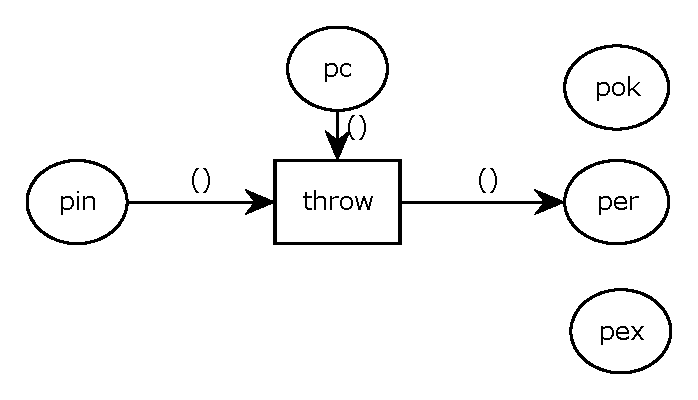
\includegraphics[scale=0.3]{Images/throw.eps}}
\hspace{0.1cm}
\subfloat[Exit PTCPN]{\label{fig:exit}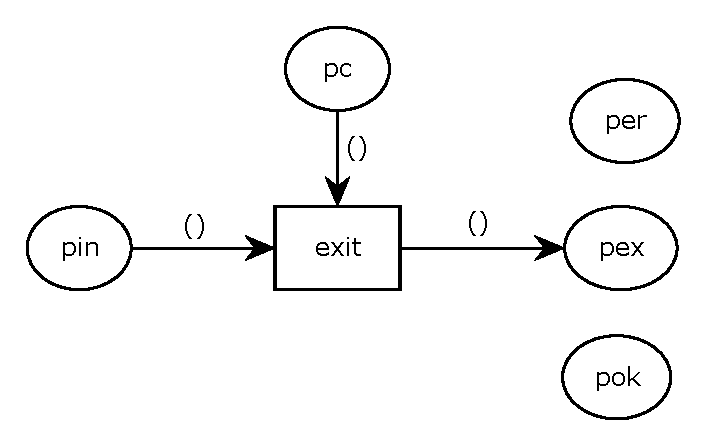
\includegraphics[scale=0.3]{Images/exit.eps}}
\hspace{0.1cm}
\subfloat[Empty PTCPN]{\label{fig:empty}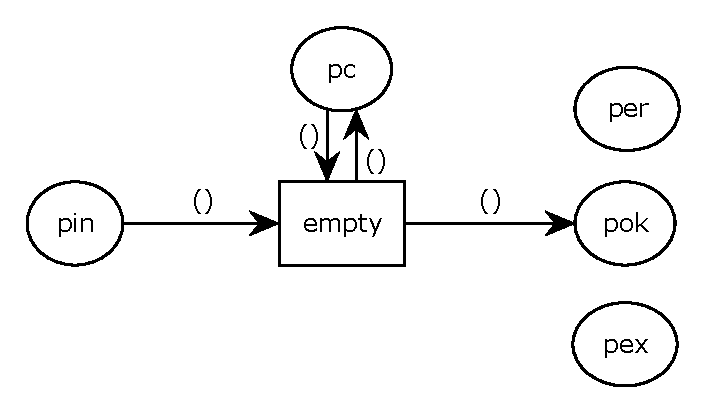
\includegraphics[scale=0.3]{Images/empty.eps}}\\
\subfloat[Wait PTCPN]{\label{fig:wait}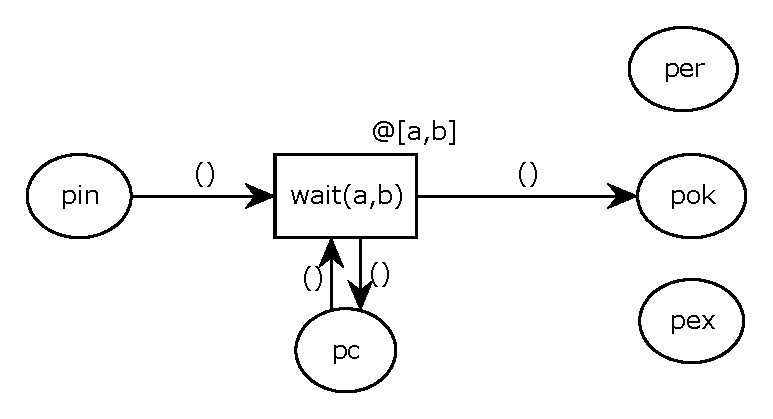
\includegraphics[scale=0.3]{Images/wait.eps}}
\ \ \ \ \subfloat[Assign PTCPN]{\label{fig:assign}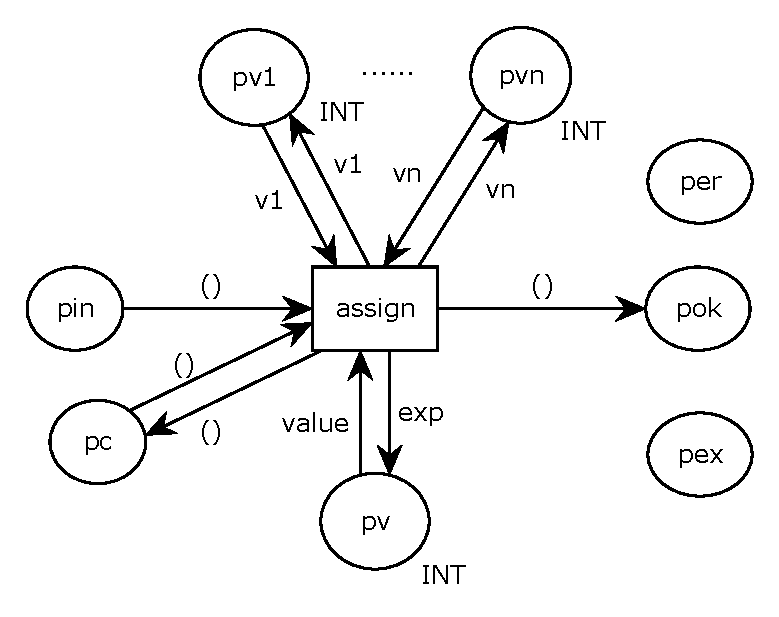
\includegraphics[scale=0.3]{Images/assign.eps}}
}}
\end{center}
\vspace{-0.5cm}
\caption{\label{fig:basicas}Basic Activities
Translation}
\vspace{-0.3cm}
\end{figure}
%\newpage

\item {\it Communication activities}:
The model we use is based on the invoke and receive operations, 
as well as the reply activity that uses a server to reply to a client. We have also added a barred version
of reply to synchronise with the response from the server. We have therefore introduced 
this last activity in our semantics to deal with the synchronous or asynchronous nature of the invoke activity (one-way or request-response operation, respectively), so the $\overline{reply}$ activity is optional in the syntax depicted in Table \ref{BPELsyntax}. 
%\vspace{-0.7cm}
\begin{figure}[!ht]
%\vspace{-0.5cm}
\hspace*{1.0cm}
\begin{center}
\fbox{ \parbox[t]{9cm}{ \center 
\subfloat[Invoke/Receive PTCPN]{\label{fig:comm1}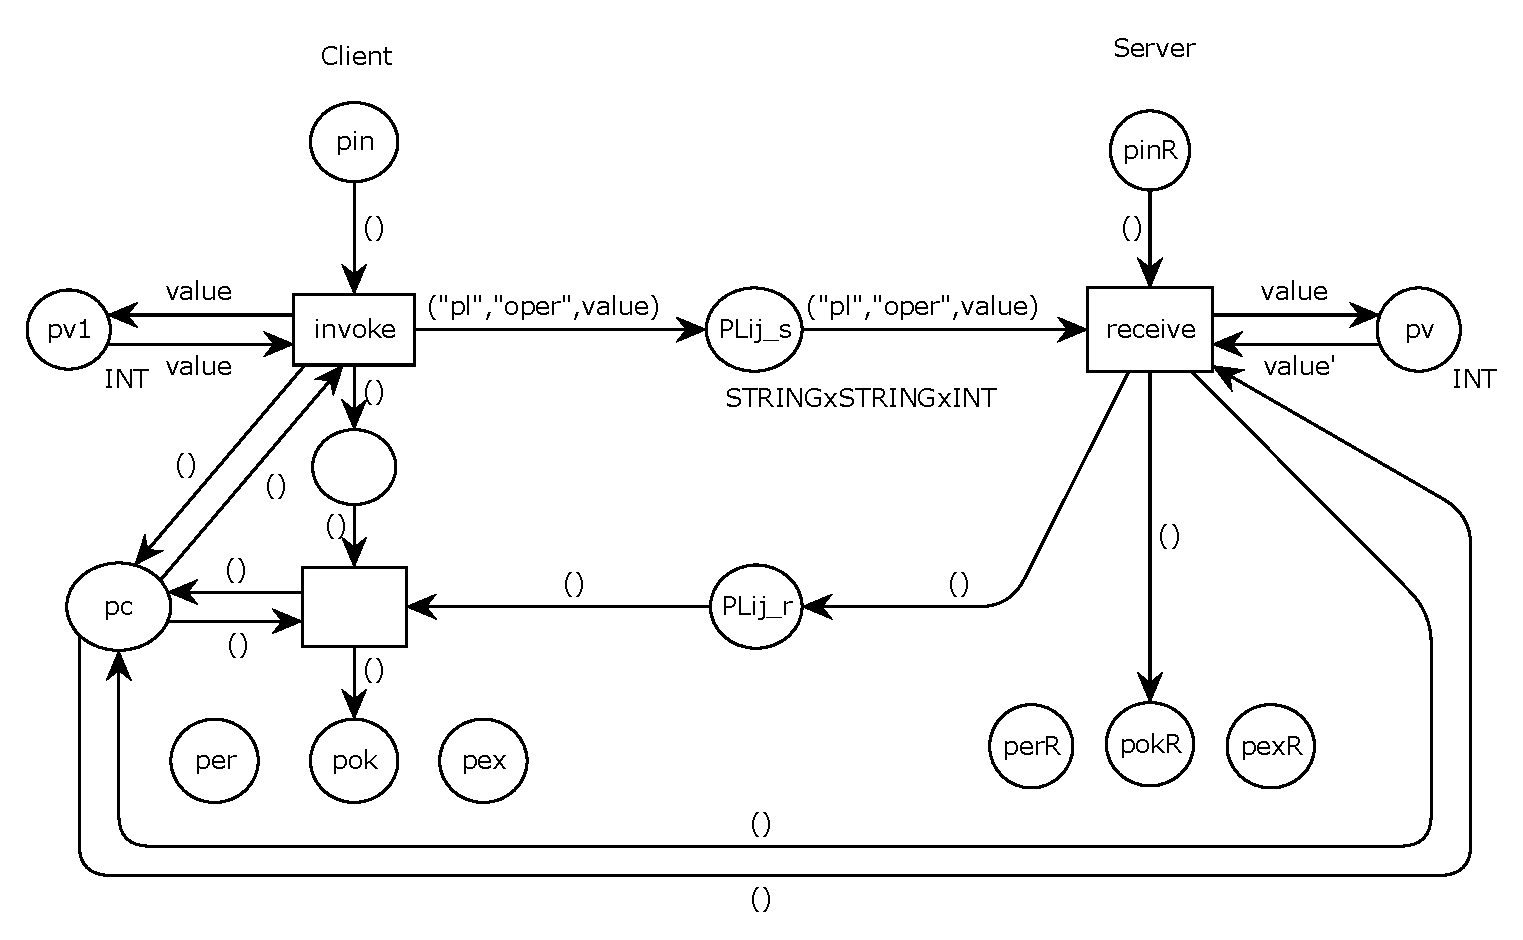
\includegraphics[scale=0.27]{Images/communication.eps}}\\
\subfloat[Reply/$\overline{Reply}$ PTCPN]{\label{fig:comm2}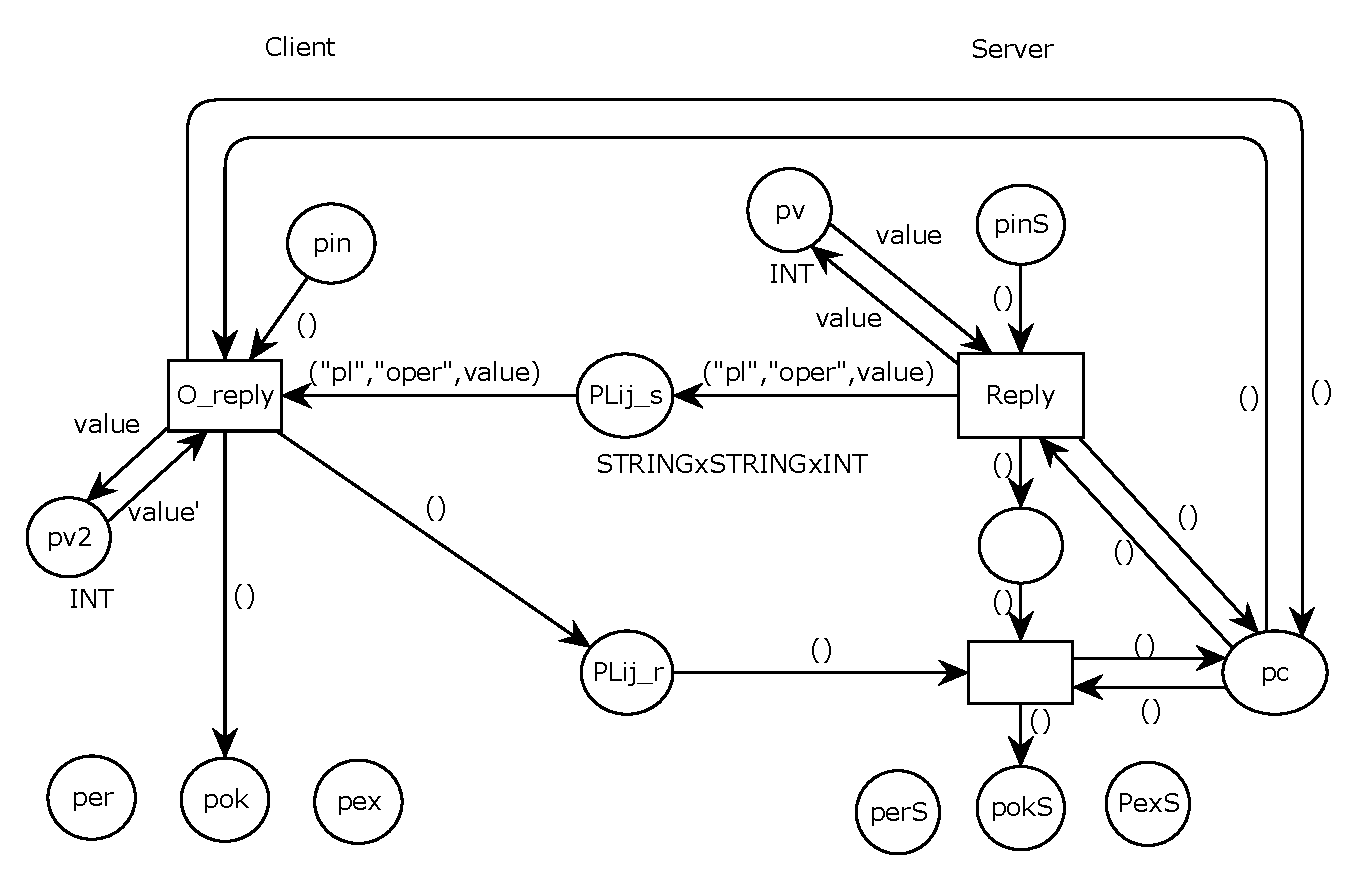
\includegraphics[scale=0.27]{Images/communication_2.eps}}
}}
\end{center}
\vspace{-0.5cm}
\caption{\label{fig:comm}Invoke/Receive Activities
Translation}% \vspace{1cm}
%\vspace{-0.5cm}
\end{figure}

%In this case, we have added to our timed Petri net two specific places in order to manage the execution of invoke/receive and reply/$\overline{reply}$, $PLij\_s$ and $PLij\_r$. Thus, we only require two places to represent all the partnerlinks between two services since we will bind each one with its corresponding counterpart by using the colours of the tokens. Place $PLij\_s$ receives tokens with three parameters: $pl,op$ and $value$, whereas $PLij\_r$ is marked only when the activity has received the data, so this place is marked with the value 0. For the sake of simplicity, we exchange only the value of the variables, but this could be easily extended to any kind of data. We depict the Petri nets in Fig. \ref{fig:comm} that express the communication among partners. In Fig. \ref{fig:comm1}, the \emph{invoke} activity extracts the value to send from the variable place ${\it P_v}$ and mark the ``sending'' partnerlink with a token endowed with this information. Once this place is marked, the receive transition can be fired marking $PLij\_r$ to allow the invoke activity to continue, and storing directly the data exchanged in the corresponding variable place. The interpretation of Fig. \ref{fig:comm2} is analogous.  
Fig.~\ref{fig:comm} shows the translation for both the invoke/receive and the reply/$\overline{reply}$ pairs of activities. Part \ref{fig:comm1} of the figure corresponds to the invoke/receive translation, in which the net of the invoke activity is depicted on the left-hand-side part, whereas the receive activity is depicted on the right-hand-side part. There are two shared places, $PL_{ij{_s}}$ and $PL_{ij{_r}}$, which are used to implement the synchronisation between the invocation and reception of services. Both places are associated to the partnerlink used for this communication, denoted here by $(i,j)$, where $i$ and $j$ are the orchestrator identifiers performing those activities. Notice that the value of a single variable is transmitted, which is obtained from the corresponding variable place, $p_v$. In the same way, the receive activity stores this value in its own variable. The interpretation of Fig.~\ref{fig:comm2} is analogous.  
\end{itemize}
%
% ======================================================================
%                            ORDERING 
%=======================================================================
\subsection{Ordering structures}

%Structured activities prescribe the order in which a collection of activities is executed. They 
%describe how a business process is created; by composing the basic activities and the WSRF-compliant activities (presented previously)
%it performs into structures that express the control patterns, handling of 
%faults and external events, and coordination of message exchanges between process instances 
%involved in a business protocol.  
WS-BPEL defines structured activities for various control-flow patterns:
\begin{itemize} 
\item Sequential control between activities is provided by $<$sequence$>$, $<$if$>$, \linebreak $<$while$>$, 
$<$repeatUntil$>$, and the serial variant of $<$forEach$>$. 
\item Concurrency and synchronization between activities is provided by $<$flow$>$ and the 
parallel variant of $<$forEach$>$.  
\item Deferred choice controlled by external and internal events is provided by $<$pick$>$.  
\end{itemize}
The set of structured activities in WS-BPEL is not intended to be minimal \cite{BPEL4WS}, so there are cases where 
the semantics of one activity can be represented using another activity. Nevertheless, in order to reduce the complexity
of our translation, our approach omits many derived activities only dealing with the most important ones from the modelling viewpoint,
such as sequence, parallel and choice. For all these cases we provide the translation
by only considering two activities. However, the generalization
to a greater number of activities is straightforward in all
of them. 
\begin{itemize}

\item {\it Sequence}\,: A sequence of two activities $A_1;A_2$ (with PTCPNs $N_{A_1}$ and
      $N_{A_2}$, respectively)
      is translated in a simple
      way (Fig.\,\ref{seq}), by just collapsing in a 
      single place (this will be
      an internal place of the new PTCPN)
      the {\it output} place $P_{ok}$ of $N_{A_1}$, and the
      {\it entry} place of $N_{A_2}$.  The {\it entry} place
      of the new PTCPN will
      be the {\it entry} place of $N_{A_1}$. The
      {\it output} place of the new PTCPN will
      be the {\it output} place of  $N_{A_2}$, and we also
      collapse the {\it exit}, {\it error} and {\it control}  places of both PTCPNs.

%\vspace{1cm}

\begin{figure}[!ht]
%\vspace{-0.5cm}
\begin{center}
\fbox{\parbox[]{6cm}{\center
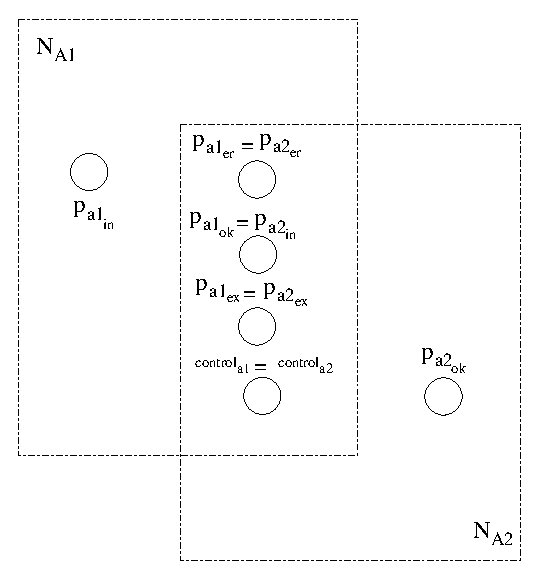
\includegraphics[scale=0.5]{Images/sequence.eps}}}
\end{center}
\vspace{-0.5cm}
\caption{\label{seq} Sequence Translation}
%\vspace{-0.6cm}
\end{figure}

\item {\it Parallel}\,: The translation for a parallel activity is depicted
in Fig.\,\ref{par}, which includes two new transitions $t1$ and
$t2$. The first to fork both parallel activities
and the second to join them when correctly terminated. 
Transition $t1$ thus puts one token on the initial places of both
PTCPNs, $N_{A_1}$ and $N_{A_2}$, in order to activate them,
and also puts one token on a new place, $p_c$, which is
used to stop the execution of one branch when the other has
failed or the exit activity is explicitly executed in one of them.
This place is therefore a precondition of every 
transition in both PTCPNs, and it is also a postcondition
of the non-failing transitions. However, in the event
of a failure or an exit activity, the corresponding {\em throw} or {\em exit}  transition
will not put the token back on $p_c$, thus
halting the other parallel activity.

Notice also that the {\em error} places of ${N}_{A_{1}}$ and $N_{A_{2}}$
have been joined in a single error place ($p_{\it er}$),
which becomes marked with one token on
the firing of one {\em throw} transition. 
In this case, the other activity cannot execute any
more actions ($p_c$ is empty), so some dead tokens would
remain permanently on some places in the PTCPN.
However, these tokens cannot cause
any damage, since the control flow has been
transferred either to the fault handling activity of the PTCPN, 
once the place $p_{er}$ has become marked, or the whole system has terminated once 
the place $p_{ex}$ is marked. %A similar reasoning is done with the {\em exit} places.
%It is a need to remark we do not treat 
%some BPEL flow construction attributes such as join conditions,
%dead path elimination, etc., since is out of the scope of this paper.
\begin{figure}[!ht]
%\vspace{-0.75cm}
\begin{center}
\fbox{\parbox[t]{12cm}
{\begin{center}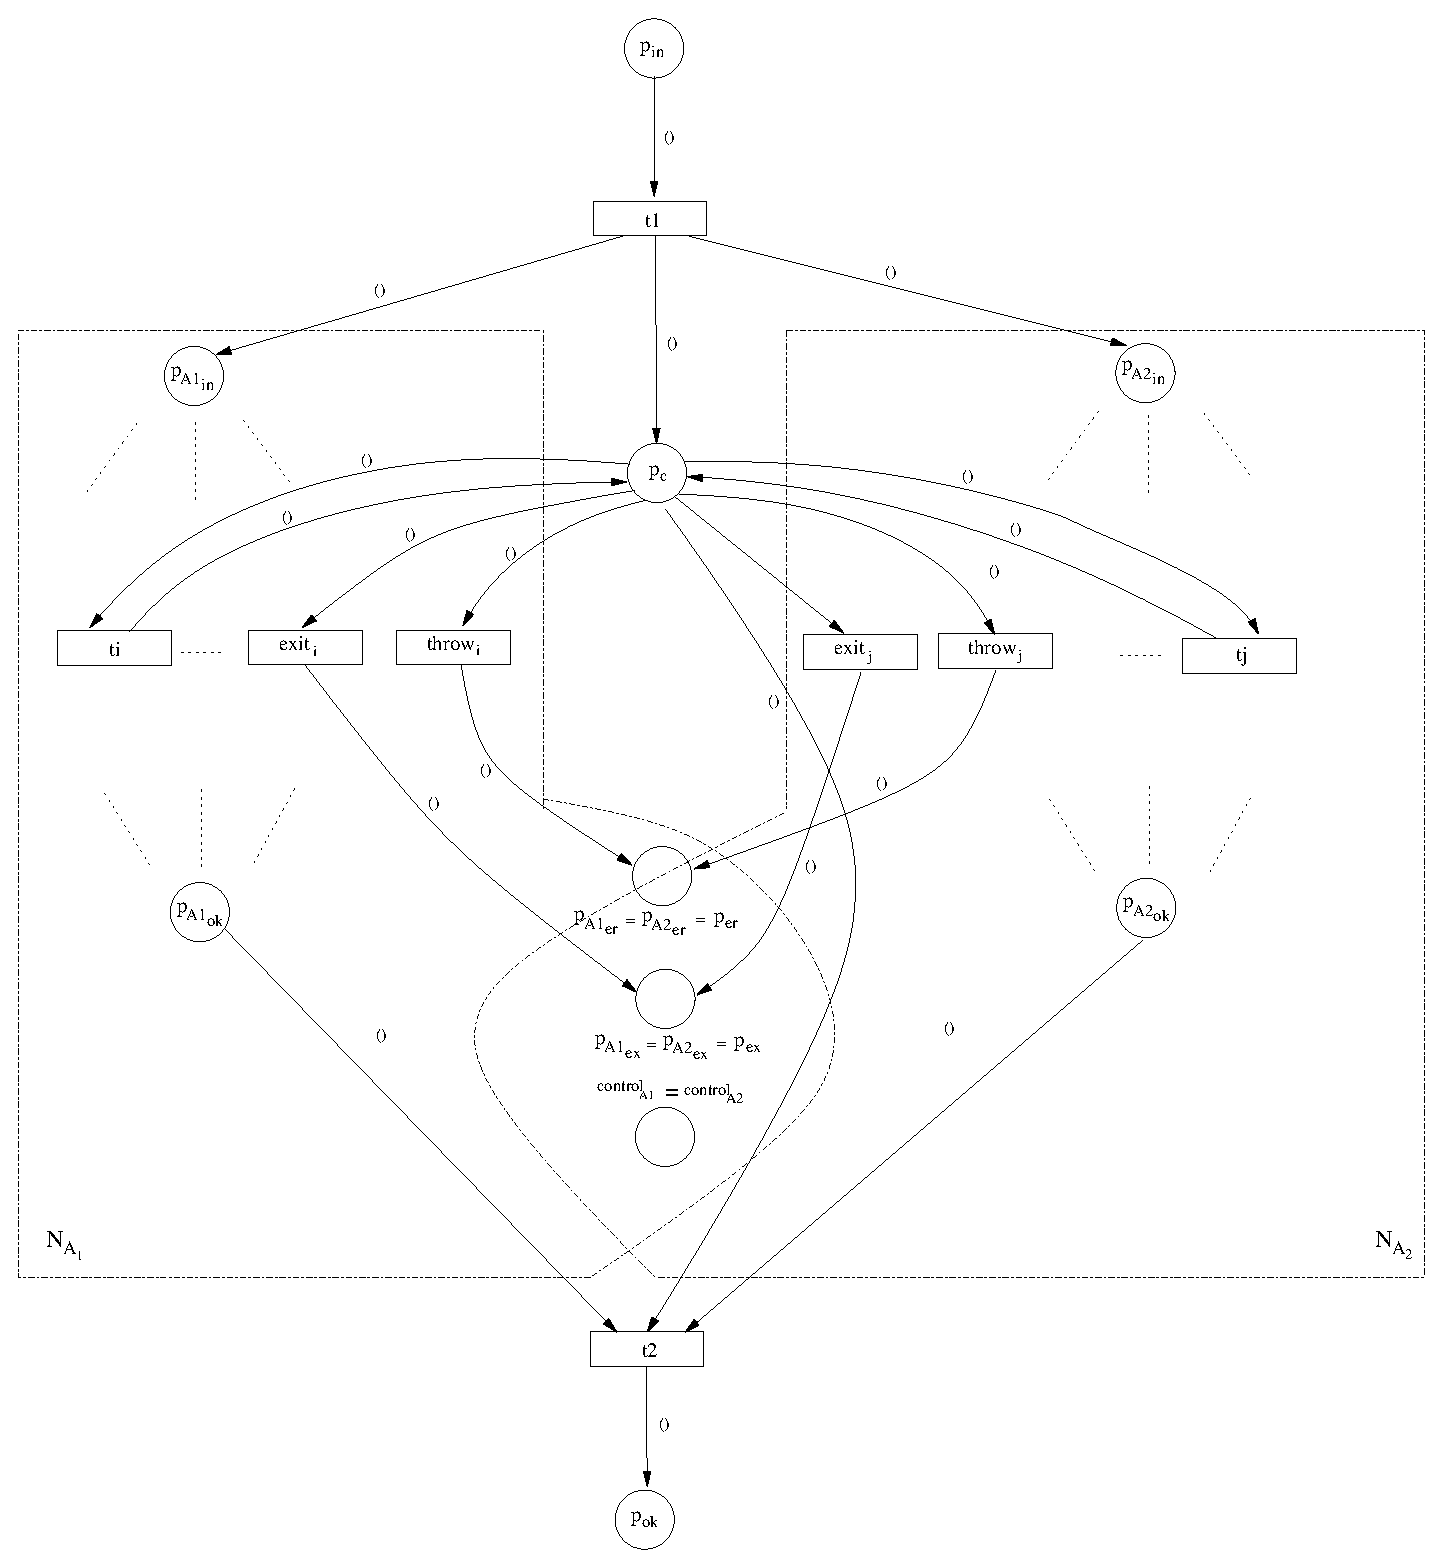
\includegraphics[height=10cm,width=12cm]
{Images/paralelo.eps}\end{center}}}
\end{center}
\vspace{-0.5cm}
\caption{\label{par} Parallel Activity Translation.}
%\vspace{-0.5cm}
\end{figure}

\item {\it Pick $(\{(pl_i,op_i,v_i,A_i)\}_{i=1}^n,A,timeout)$}: The $<$pick$>$ activity waits for the occurrence of exactly one event from a set of events, also establishing a
time-out for this selection. The translation is depicted in Fig.~\ref{pick} where a timer is implemented on the place {\it p\_a} in order to enforce the firing of transition {\it ta} when the timeout has elapsed, thus activating {\it N$_{A}$}. The colour set {\it INT} of {\it p\_a} is timed.  To illustrate how this construction works, we define the following example.
\begin{example}
In this example, there are three actors: two customers and a seller. The customers contact the
seller in order to gather information about a specific product identified by id1 and id2, respectively. The seller checks the
stock and send the requested information to the customers. The seller has established a timeout of 24 hours to receive requests. Let the orchestrations $O_{c1}=({pl_1},{id_1,id_3},A_{c1} , empty)$, $O_{c2} = ({pl_2},{id_2,id_4},A_{c2},$ $empty)$ and $O_{s} = ({pl_1,pl_2}, {id_{s1},id_{s2}, inf_{s1},inf_{s2}},A_s , empty)$ , the BPEL+ WSRFN code for the primary activity of both participants is:\\
\[\begin{array}{l}
A_{c1} = invoke(pl_1 , info, id1 ); receive(pl_1 , inforec1, id_3 ) \\
A_{c2}= invoke(pl1 , info, id1 ); receive(pl_2 , inforec2, id_4 ) \\
A_s = pick(\{(pl_1,info,id_{s1},reply(pl_1 , inforec1, id_3),(pl_2,info,id_{s2},\\
\hspace{0.9cm} reply(pl_2 , inforec2, id_4))\},empty,24)
\end{array}\]
\end{example}
\begin{figure}[!ht]
%\vspace{-0.5cm}
\begin{center}
\fbox{\parbox[c]{11.3cm}{\begin{center}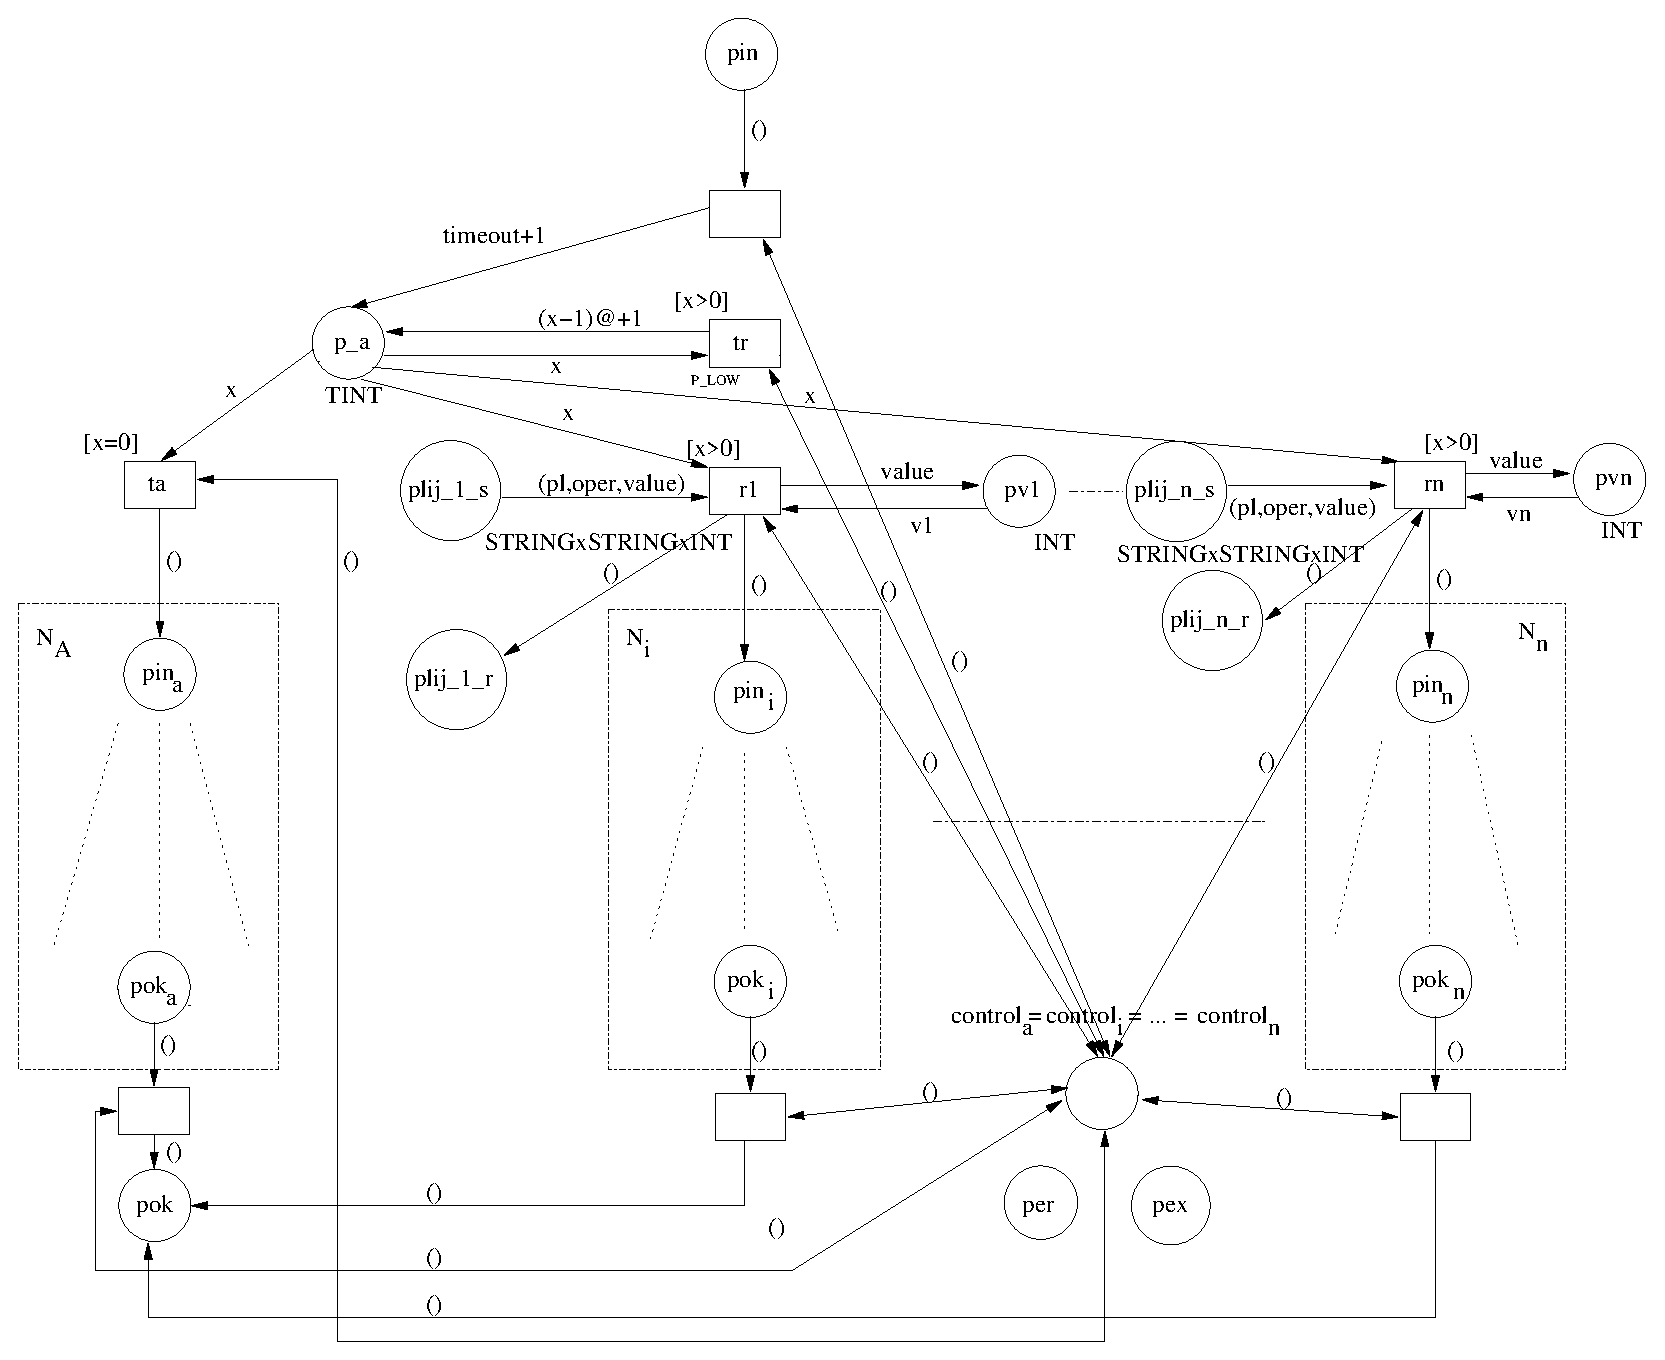
\includegraphics[scale=0.4]
{Images/pick.eps}\end{center}}}
\end{center}
\vspace{-0.5cm}
\caption{\label{pick} Pick Activity Translation.}
%\vspace{-0.4cm}
\end{figure}
Looking at Fig. \ref{pick}, it can be observed that when ${\it O_s}$ executes the \emph{pick} activity the input place ${\it p_{in}}$ of the net is marked. Next, transition ${\it t_{in}}$ is fired in order to mark the place ${\it p_a}$ with the value $timeout+1$. Two situations can then occur. One of the buyers may perform its {\emph invoke} activity before the timeout expiration, putting a token in the corresponding input place, ${\it plij_{i{_s}}}$ of the transition ${\it r_i}$, $i \in {1,..,n}$, and, then, the behaviour hereafter is the same as in the {\it receive} activity (Fig. \ref{fig:comm}). On the other hand, if none of the buyers executes an \emph{invoke} activity, the current time is increased by firing the transition ${\it t_r}$. This transition is enabled until the timeout is reached, that is, the value of $x$ is equal to 0. In that case, the PTCPN corresponding to activity $A$ is performed. We have used variable $x$ as a countdown timer due to a restriction of CPNTools, which does not allow to include the \emph{time} function in guards since its inclusion could pose side-effects\cite{CPNTools}.  
%The time delay inscription of the arc from ${\it t_r}$ to ${\it p_a}$ is necessary since CPNTools only evaluates 
%The $<$pick$>$ activity completes when the selected activity finishes.
%, then 
%executes the activity associated with that event. After an event has been selected, the other events 
%are no longer accepted by that $<$pick$>$. The $<$pick$>$ activity is comprised of a set of branches, each containing an event-activity pair.  
 %The activities contained in this construction can come in two forms: 

%\begin{itemize}
%\item The $<$onMessage$>$ is similar to a $<$receive$>$ activity, in that it waits for the receipt of an 
%inbound message. 
%\item The $<$onAlarm$>$ corresponds to a timer-based alarm. If the specified duration value 
%is zero or negative, or a specified deadline has already been reached or 
%passed, then the $<$onAlarm$>$ event activity is executed immediately. 
%\end{itemize} 
% must act in a similar fashion, but adding a feature
%which permits the selection among some activities. This selection is easy to model with Petri nets since collapsing the input places of the possible branches
%it is impossible to execute more than one at the same {\em pick}. In our model, the place {\em PinA1..An} represents this behaviour. Finally, in the BPEL specification, 
%is encouraged the use of time-outs with {\em pick} activity, so we have included a timed transition with its corresponding timed guard in order to manage the execution of 
%an ``alarm activity'' only in the event the time-out expires. The meaning of the other places and transitions is the same as in the receive activity.  

\item {\it While(cond,A)}: The machinery needed to model this construction is fairly straightforward since we only must check if the repetition condition holds or not in order to execute the contained activity or skip it. Fig.~\ref{while} shows this translation.
\end{itemize}
%The $<$while$>$ activity provides for repeated execution of a contained activity. The contained 
%activity is executed as long as the boolean condition evaluates to true at the beginning of 
%each iteration. The meaning of the places and transitions of the net represented in Fig. \ref{while} is fairly straightforward, so, due to space limitations, we are going to omit any explanation of its elements. 
%The meaning of the places and transitions are fairly straightforward, so, due to space limitations, we are going to omit any explanation of the elements contained in this net 
%\newpage


%\vspace{-1.3cm}

\begin{figure}[!ht]
%\vspace{-0.7cm}
\begin{center}
\fbox{\parbox[t]{11.3cm}{\begin{center}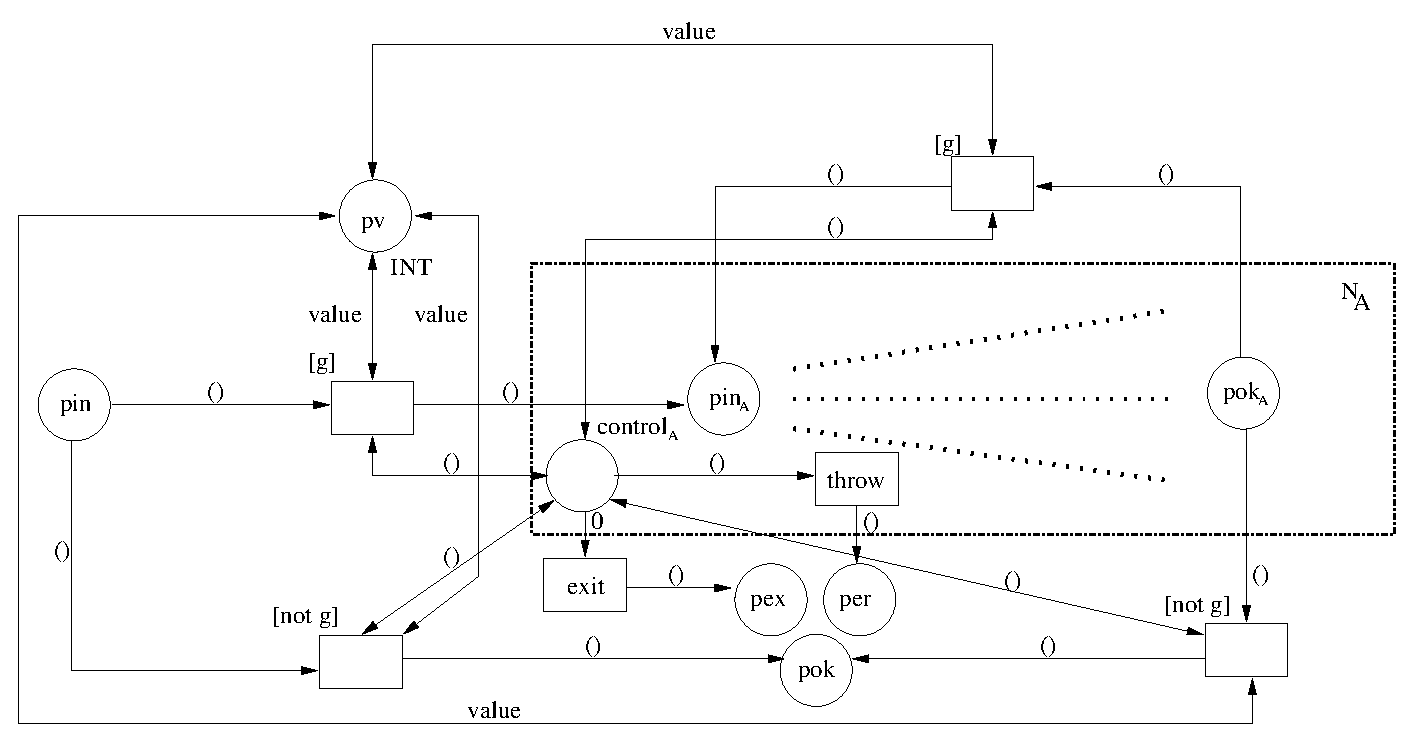
\includegraphics[scale=0.4]
{Images/while.eps}\end{center}}}
\end{center}
\vspace{-0.5cm}
\caption{\label{while} While Activity Translation.}
%\vspace{-0.7cm}
\end{figure}
\vspace{-0.5cm}
% ======================================================================
%                            WSRF 
%=======================================================================
\subsection{WSRF/WSN compliant}
%In this section, we state the WSRF activities we have integrated with the BPEL activities in order to create a framework for modelling stateful workflows. It is worth noting that in recent years have appeared a new redefinition of workflow nets which deals with resources called Resource-Constrained Workflow Nets \ref{}. As commented in the Related Work section, this approach extends the well-known formalism, Workflow nets, with finite resources such as money, memory and so on, but the authors do not provide the machinery
%to create and destroy such resources, so this extension of Workflow nets matches with the idea of WSRF standard, i.e., the creation and destruction of resources is out of the scope of the specification. Nevertheless, our approach was devised to manage the whole lifetime of the resource from its creation until its destruction.


%To date, we have presented the activities corresponding to the ``BPEL'' activities part of our model. Next, we will state the counterpart of our approach, i.e., the activities, which permit the creation and modification of the resources as well as the management of the subscriptions to them following the indications of the standard WSRF. Notice that a novelty in our model is the creation of resources since WSRF does not specify how this creation is done.
%\begin{figure}[!ht]
%\vspace{-0.5cm}
%\begin{center}
%\fbox{\parbox[t]{12cm}{\begin{center}\includegraphics[scale=0.35]
%{Images/createResource.eps}\end{center}}}
%\end{center}
%\vspace{-0.7cm}
%\caption{\label{createresource} CreateResource Activity Translation.}
%\vspace{-1.5cm}
%\end{figure}

%To begin with, we depict the creation of resources in Fig. \ref{createresource}. In order to guarantee our PTCPNs are 1-safe, we opted as commented above to model each resource with two dedicated places,  $p_{\it r_i}$, and $p_{\it r_a}$, which represent the possible state of the resources, instantiated or not instantiated, respectively. Thus, when an orchestrator wants to create a resource, the firing of the transition {\it createResource} moves the token from the ``inactive'' ($p_{\it r_i}$) to the ``active'' place ($p_{\it r_a}$) making available this resource to the subscribers. Once the place $p_{\it r_a}$ is marked and an orchestrator executes the activity {\em subscribe}, our translation can automatically build the subscriptions nets. Here, a subscription net is formed by a transition, whose guard is the subscription condition, and the subnet which corresponds to the translation of the activity that the subscriber wants to be executed just in case the subscription condition ${\it gc_i}$ holds. Notice that WSRF allows the creation of multiple subscriptions to the same resources by the same orchestrator, so we will allow this restriction. Despite the {\em subscribe} construction will be presented later, just comment here we have endowed each resource with a list that represents its subscribers with their {\em id} and an integer, $0$ or $1$, to denote whether the orchestrator with identifier {\em id} is subscribed or not. Finally, in the leftmost part of Fig. \ref{createresource}, we depict the net that will be fired in the event of the resource lifetime expires. In this situation, we return the token from the active place to the inactive place and immediately execute the activity {\em $Activity_timeisup$}, which will be passed as an argument of the {\em createResource} activity. This argument is not included in the WSRF specification, but we have incorporated it to show the benefits of the integration of both standards.       

%Now, we describe the PTCPNs who corresponds to the manipulation of resource value and lifetime as well the subscription to a specific resource. On the left side of Fig. \ref{fig:getproperty},
%the PTCPN for the activity {\em getProperty} is depicted. Here, the resource {\em value} obtained from $p_{\it r_a}$ is stored in the place of the corresponding variable. The reasoning done in the construction of the PTCPNs for the activities {\em setProperty} and {\em setTimeout} in Fig. \ref{fig:setproperty} is quite similar, but updating the resource value or its lifetime, respectively. Important to note that if an orchestrator is trying to access to a resource not instantiated, the fault place  $p_{\it er}$ will be marked starting the execution of the fault activity. 
%\begin{figure}[!ht]
%\vspace{-0.5cm}
%\hspace*{1.0cm}
%\begin{center}
%\fbox{ \parbox[t]{12cm}{ \center
%  \subfloat[GetProperty and Subscribe Activities]{\label{fig:getproperty}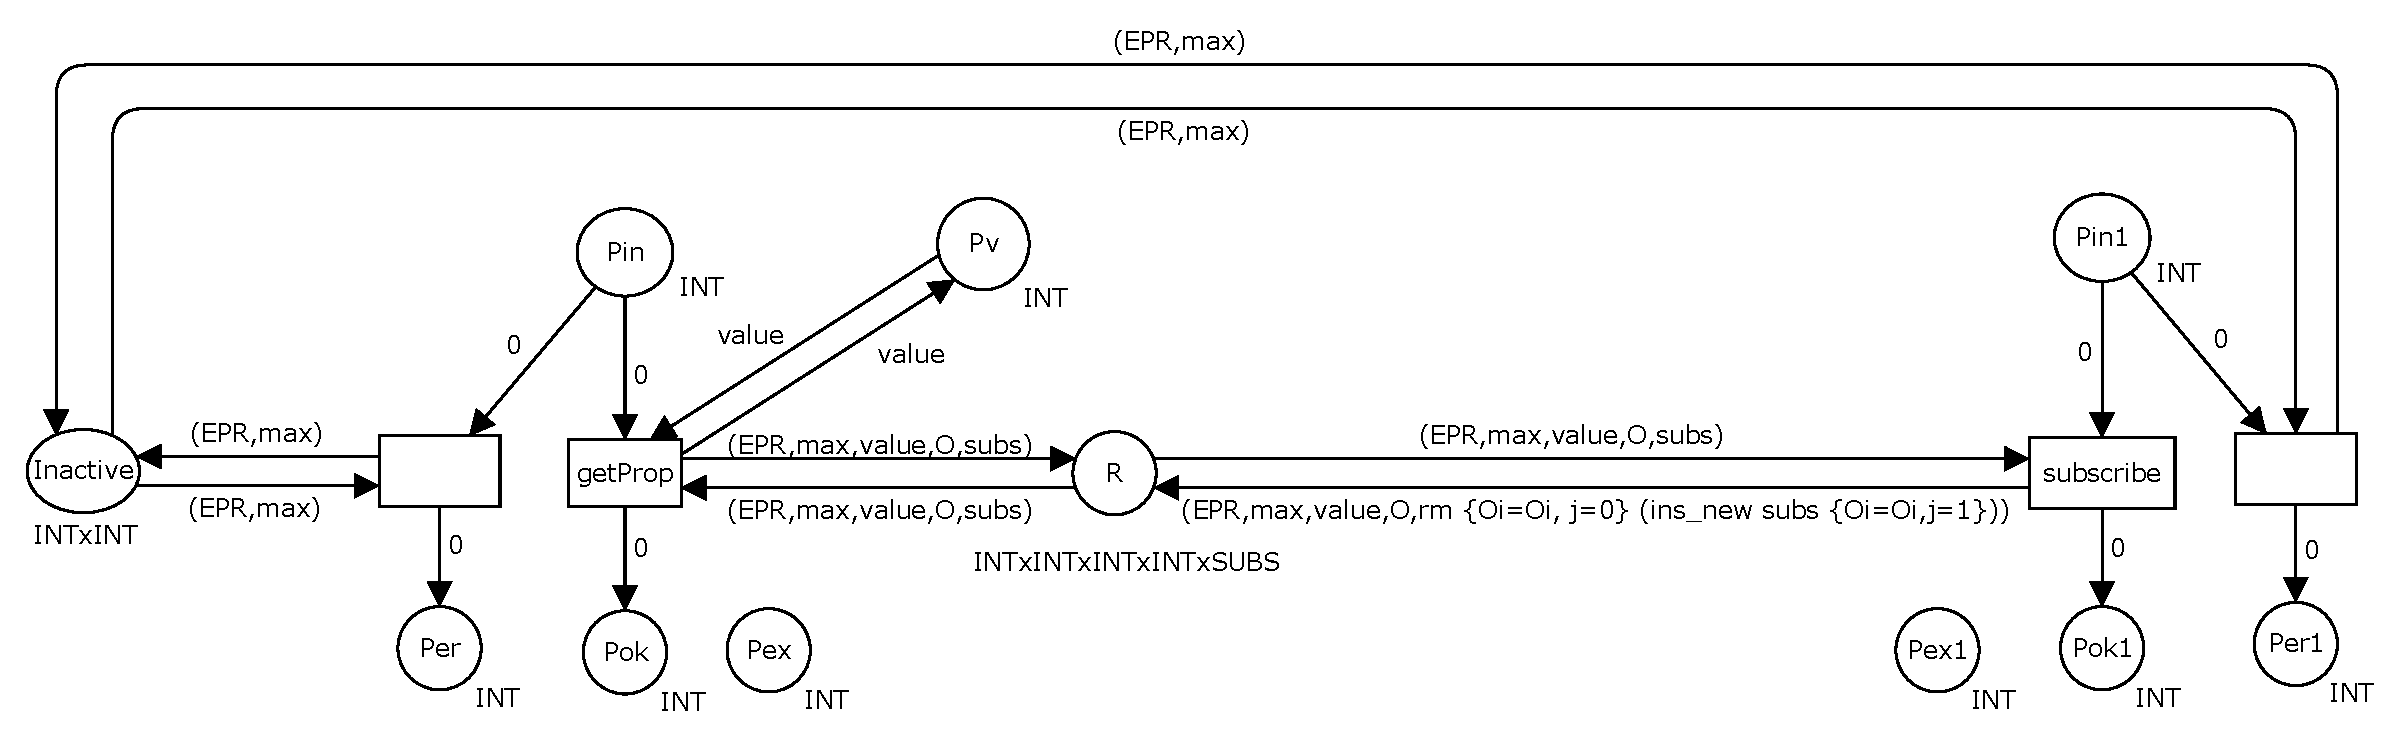
\includegraphics[scale=0.3]{Images/getProp+subscribe.eps}}\\
 % \subfloat[SetProperty and SetTimeout Activities]{\label{fig:setproperty}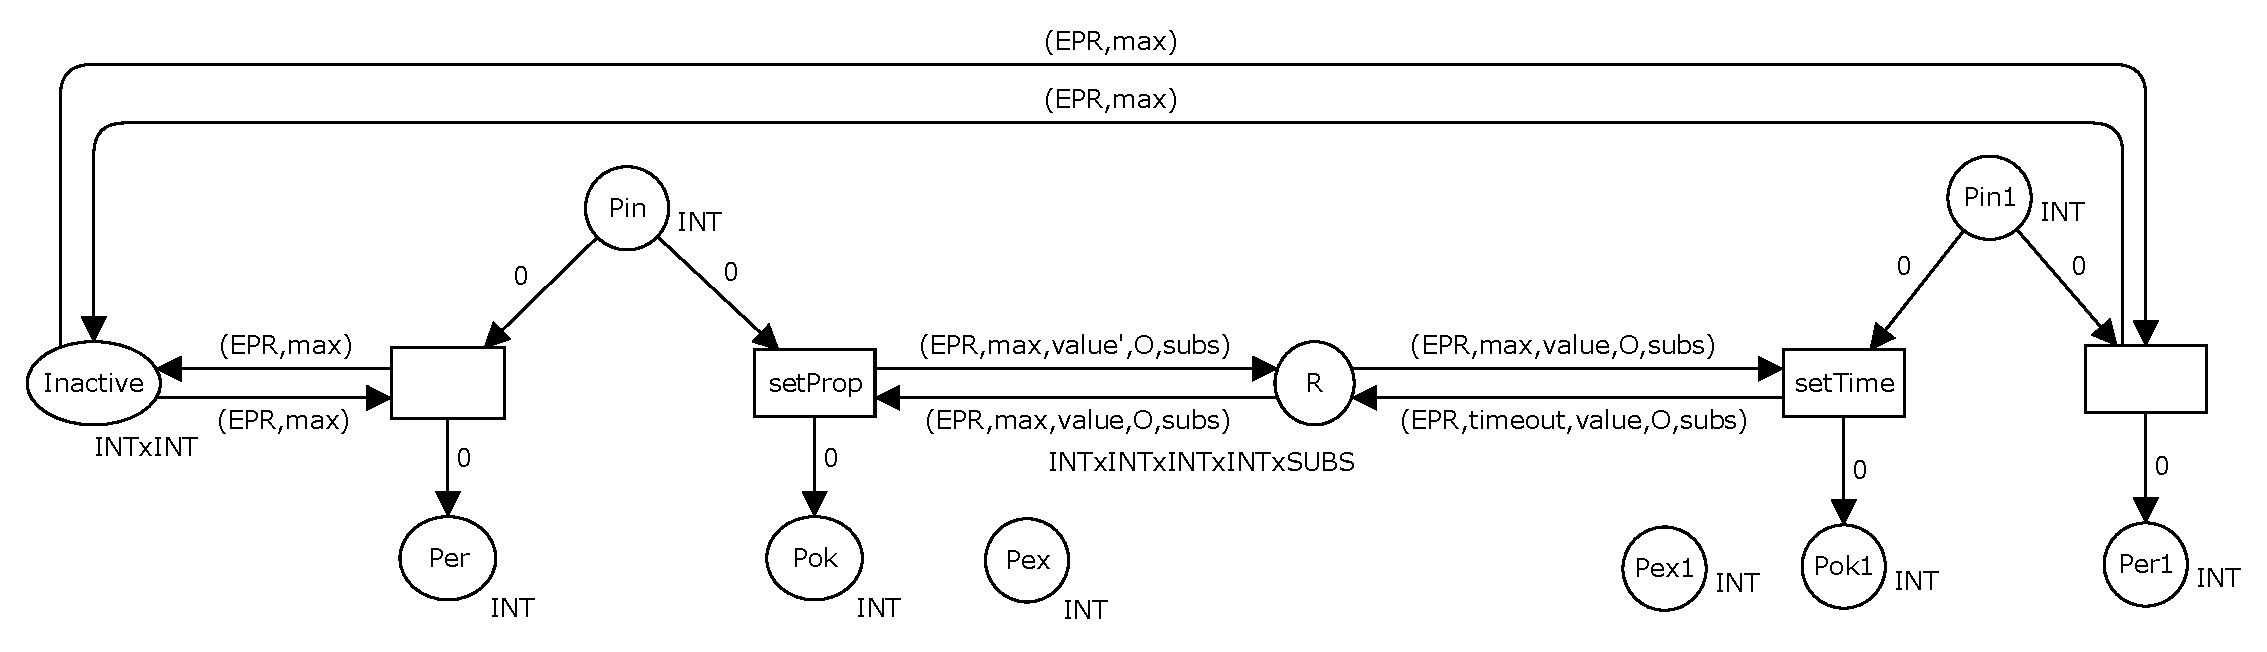
\includegraphics[scale=0.32]{Images/setProp+setTime.eps}}
 % }}
%\end{center}
%\vspace{-0.6cm}
%\caption{\label{fig_wsrf}WSRF Activities
%Translation}
%\vspace{-0.5cm}
%\end{figure}

%Finally, on the right side of Fig. \ref{fig:getproperty}, we show the PTCPN for the {\em subscribe} activity. Above, we have commented we have used a list to represent the subscribers of a resource. Since we have used CPNtools to build our nets, this ``registration stamp'' is modeled by using the record colour set provided by this tool. This record contains the identifier of the subscriber, {\em ID}, and integer variable {\em j}, whose value will be $0$ when the orchestrator is not subscribed and $1$ in the opposite case. This value will be checked in the guard of the first transition of the subscription net within the condition specified here in order to check if the orchestrator is subscribed and the condition holds. As in the previous cases, we run the fault activity if one orchestrator is trying to subscribe to non-instantiated resource.   

%\begin{figure}[!ht]
%\begin{center}
%\fbox{\parbox[t]{12cm}{\begin{center}\includegraphics[scale=0.35]
%{Images/setProp.eps}\end{center}}}
%\end{center}
%\vspace{-0.7cm}
%\caption{\label{setp} GetProperty Activity Translation.}
%\end{figure}

%\begin{figure}[!ht]
%\begin{center}
%\fbox{\parbox[t]{12cm}{\begin{center}\includegraphics[scale=0.35]
%{Images/getProp.eps}\end{center}}}
%\end{center}
%\vspace{-0.7cm}
%\caption{\label{setp} SetProperty Activity Translation.}
%\end{figure}

%\begin{figure}[!ht]
%\begin{center}
%\fbox{\parbox[t]{12cm}{\begin{center}\includegraphics[scale=0.35]
%{Images/setTime.eps}\end{center}}}
%\end{center}
%\vspace{-0.7cm}
%\caption{\label{settim} SetTimeout Activity Translation.}
%\end{figure}

%=============================Valent�n================================
Let us now see the WSRF/WSN activities, and their corresponding translations.

\begin{itemize}
\item {\it CreateResource(EPR,val,timeout,A)}:
{\em EPR} is the resource identifier, for which we have two complementary places in Fig.~\ref{createresource}, ${\it p_{r_i}}$ and ${\it p_{r_a}}$, where the sub-index represents the state of the resource: $i$ when it is inactive and $a$ when it is active. The initial value is $val$, and $A$ is the activity that must be executed when the time-out indicated as third parameter has elapsed.

We can see in Fig.~\ref{createresource} how the transition $createResource$ removes the token from the {\em inactive} place, and puts a new token on the active place, whose colour contains the following information: resource identifier (EPR), its lifetime (max), and its value (val). %the owner (O) and the list of subscribers (initially, empty).
\begin{figure}[!ht]
%\vspace{-0.7cm}
\begin{center}
\fbox{\parbox[t]{10cm}{\begin{center}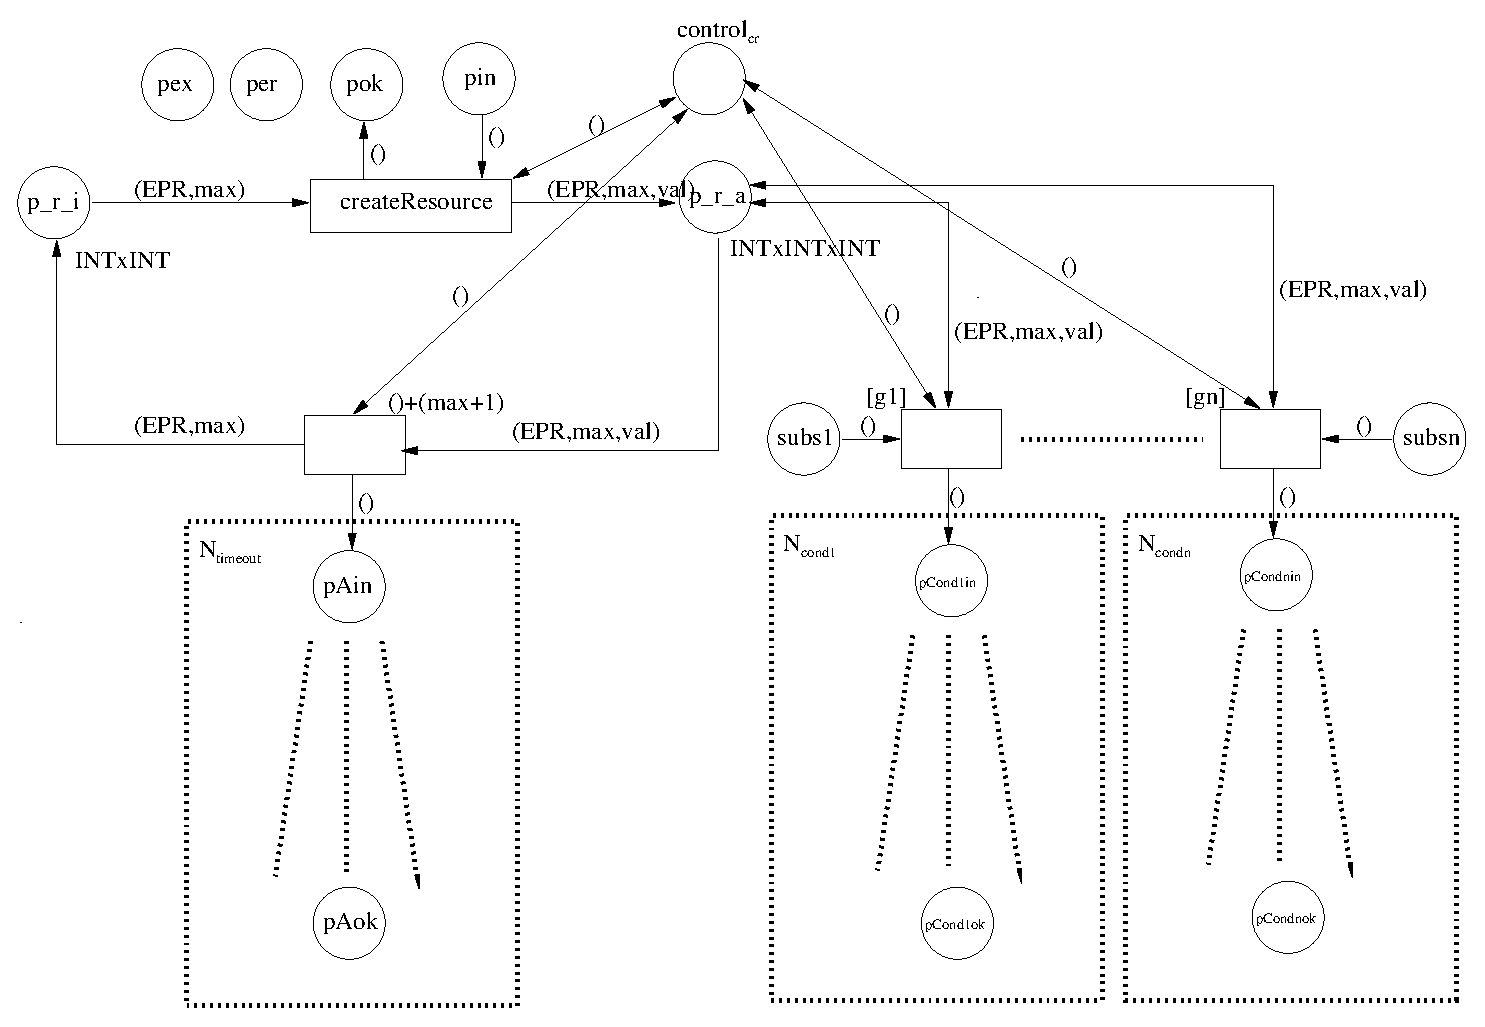
\includegraphics[scale=0.35]
{Images/createResource.eps}\end{center}}}
\end{center}
\vspace{-0.5cm}
\caption{\label{createresource} CreateResource Activity Translation.}
%\vspace{-0.5cm}
\end{figure}
Transition ${\it t}$0 is executed when the lifetime of the resource has expired, thus removing the token from the {\em active} place, marking again the {\em inactive} place, and activating $N_A$. We can also see that the {\em active} place is linked with a number of transitions, which correspond to the subscribers (we know in advance these possible subscribers from the BPEL+WSRFN document). These transitions can only become enabled if the corresponding places $subs_{i}$ are marked by performing the corresponding  activity {\em subscribe}. The PTCPNs ${\it Ncond_i}$ are the nets for the activities passed as parameter in the invocation of a subscribe activity.   
\item {\it Subscribe(EPR,cond$'$,A)}:
In this case, an orchestrator subscribes to the resource $EPR$, with the associated condition $cond'$, upon which the activity $A$ must be performed. Fig.~\ref{subscribe} shows this translation, where we can observe that the associated place $subs_{i}$ is marked in order to allow the execution of the PTCPN for the activity $A$ if the condition $g_{i}$ holds. On the contrary, if the resource is not active, we will throw the fault handling activity.
%\begin{figure}[!ht]
%\vspace{-0.5cm}
%\hspace*{1.0cm}
%\begin{center}
%\fbox{ \parbox[t]{12cm}{ \center
%  \subfloat[GetProperty and Subscribe Activities]{\label{fig:getproperty}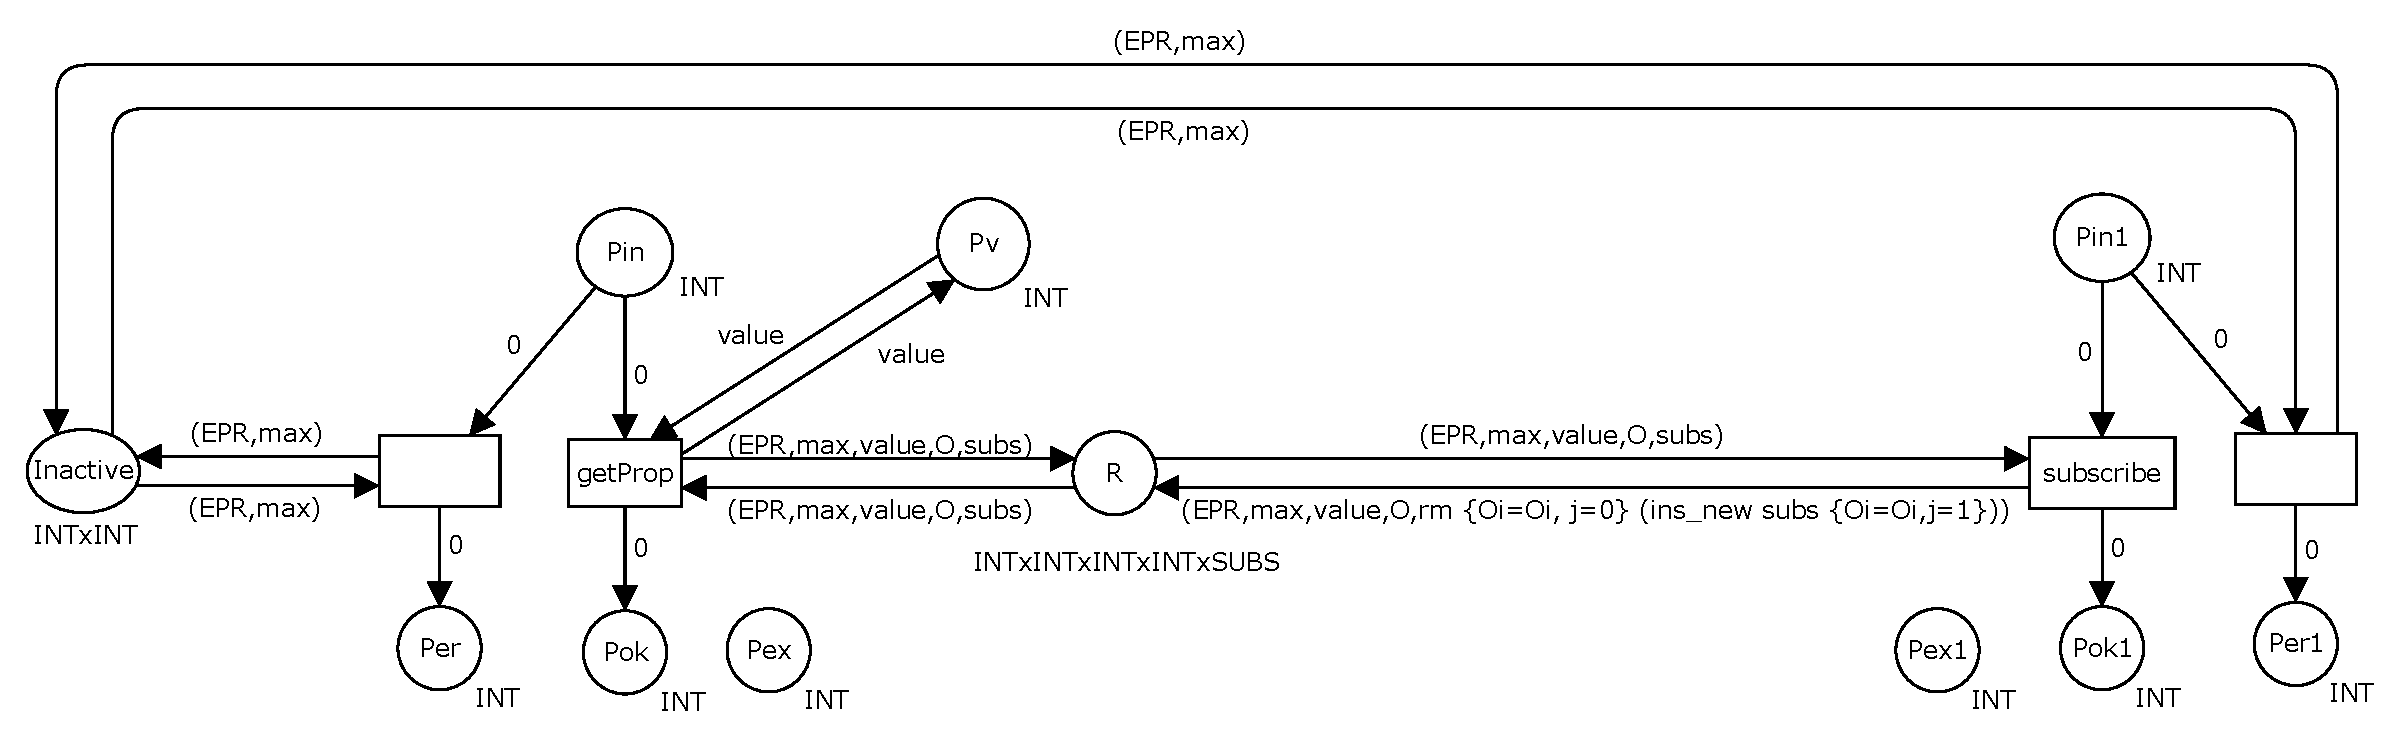
\includegraphics[scale=0.3]{Images/getProp+subscribe.eps}}\\
 % \subfloat[SetProperty and SetTimeout Activities]{\label{fig:setproperty}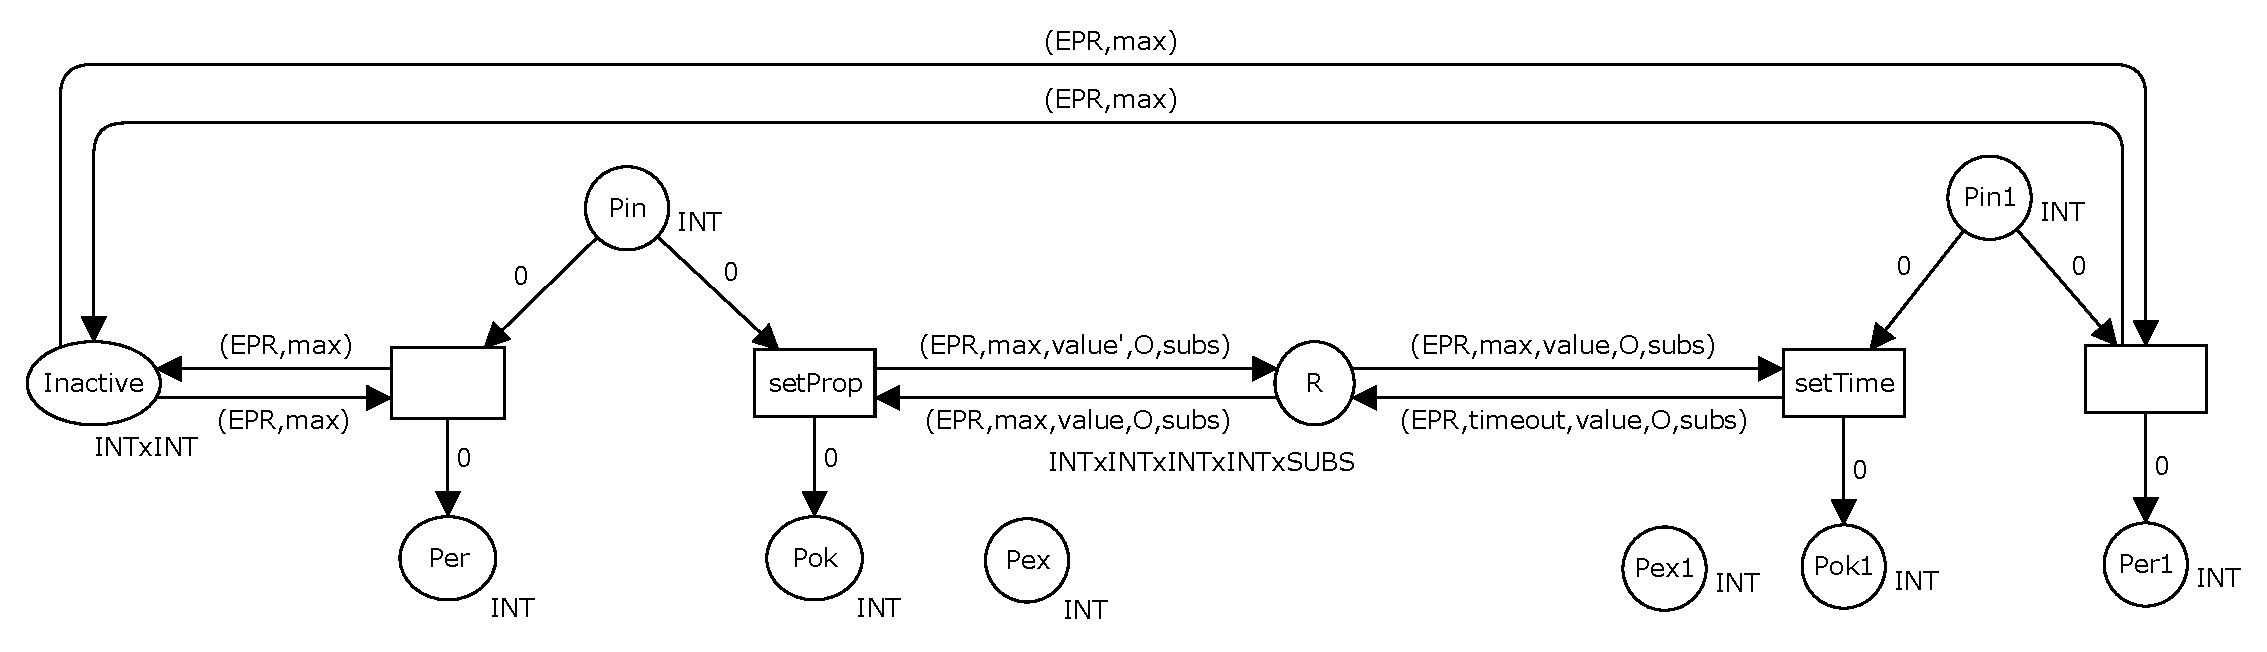
\includegraphics[scale=0.32]{Images/setProp+setTime.eps}}
 % }}
%\end{center}
%\vspace{-0.6cm}
%\caption{\label{fig_wsrf}WSRF Activities
%Translation}
%\vspace{-0.5cm}
%\end{figure}
%\newpage
\item \it{GetProp(EPR,v)} and \it{SetProp(EPR,expr)}:
These are easily translated, as shown in Figs.~\ref{getp} and \ref{setp}, where the resource value is obtained and assigned to variable $v$ (\textit{GetProp}), or a new value is assigned to the resource (\textit{SetProp}).
%\vspace{-0.8cm}

\begin{figure}[!ht]
%\vspace{1cm}
\begin{center}
\fbox{\parbox[t]{8.5cm}{\begin{center}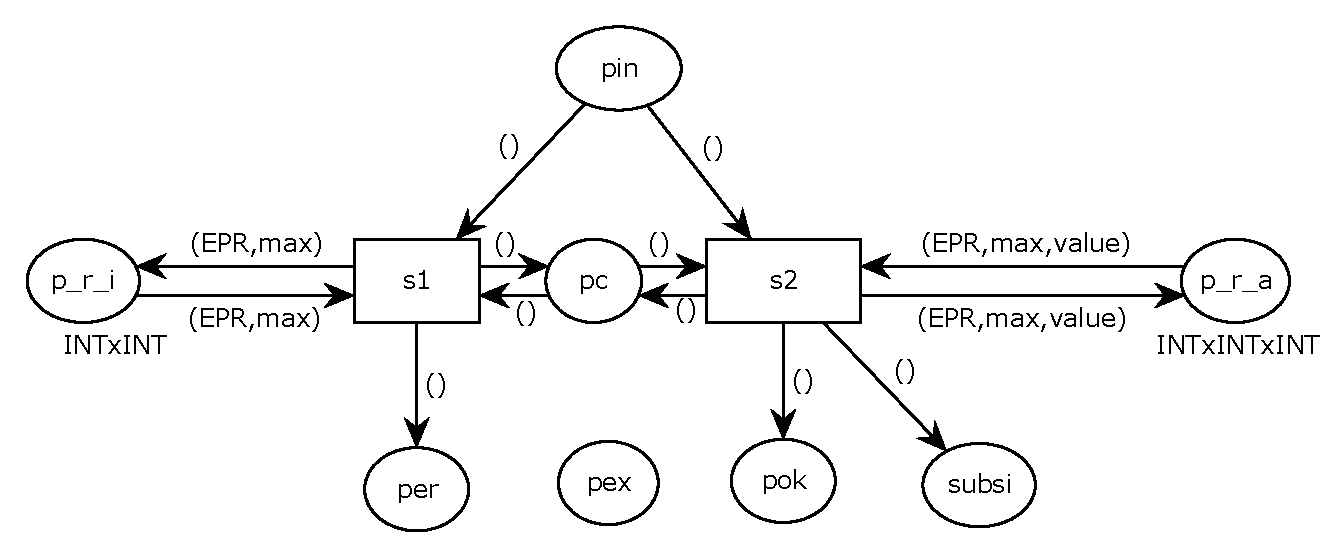
\includegraphics[scale=0.35]
{Images/subscribe.eps}\end{center}}}
\end{center}
\vspace{-0.5cm}
\caption{\label{subscribe} Subscribe Activity Translation.}
\vspace{-0.1cm}
\end{figure}

\begin{figure}[!ht]
\begin{center}
\fbox{\parbox[t]{8.5cm}{\begin{center}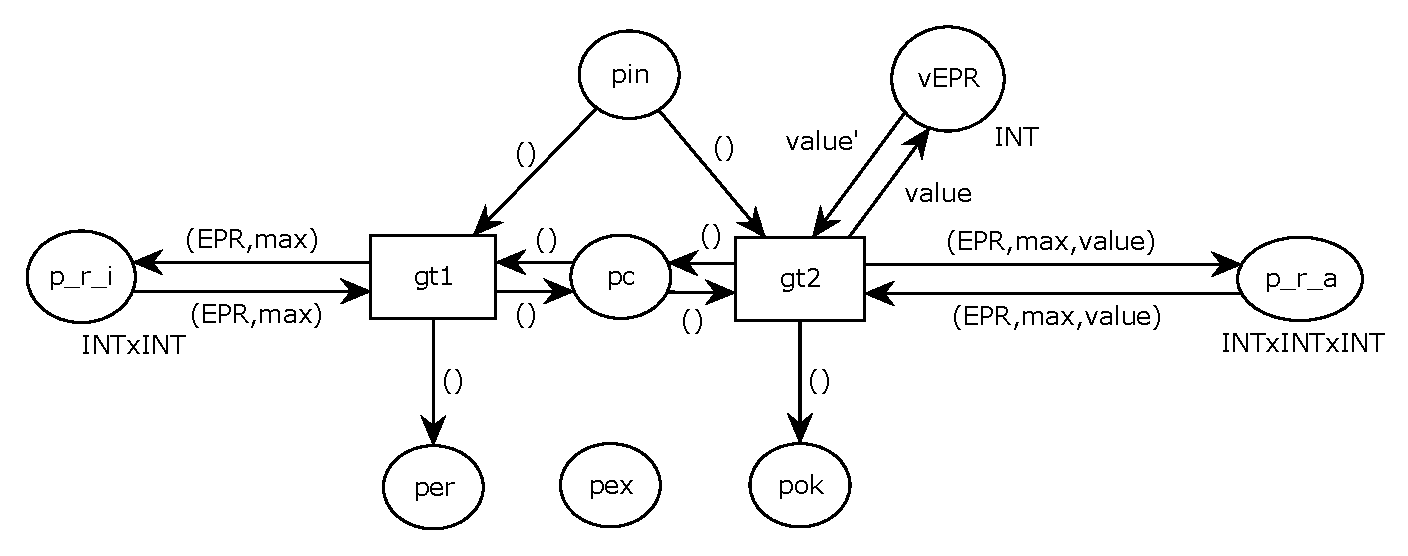
\includegraphics[scale=0.35]
{Images/getProp.eps}\end{center}}}
\end{center}
\vspace{-0.5cm}
\caption{\label{getp} GetProperty Activity Translation.}
%\vspace{-0.7cm}
\end{figure}
%\begin{figure}[!ht]
%\vspace{-0.5cm}
%\hspace*{1.0cm}
%\begin{center}
%\fbox{ \parbox[t]{11cm}{ %\center 
%\hspace{-0.2cm}\subfloat[GetProperty Activity %Translation.]{\label{fig:get}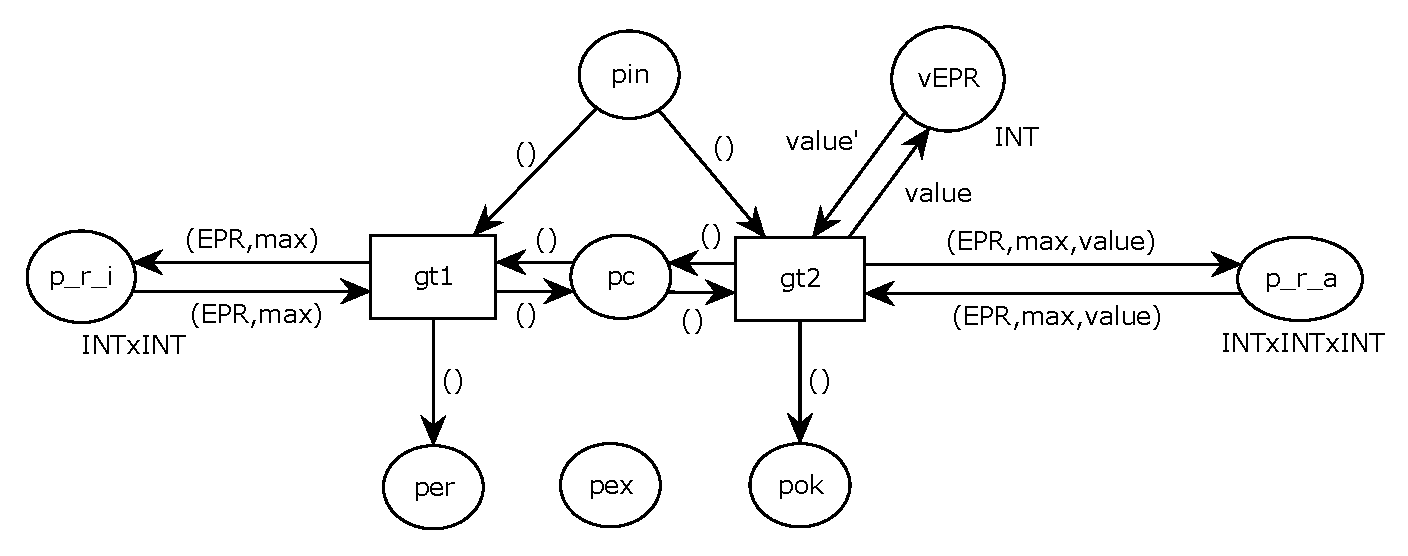
\includegraphics[scale=0.4]{Images/getProp.eps}}\\
%\subfloat[SetProperty Activity %Translation]{\label{fig:set}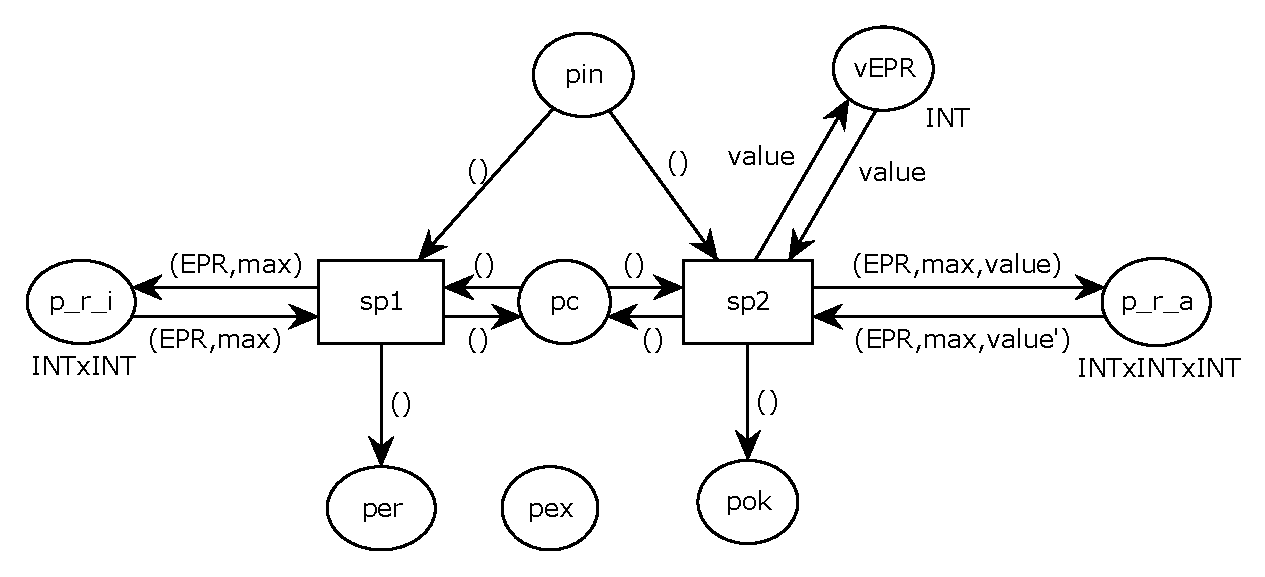
\includegraphics[scale=0.4]{Images/setProp.eps}}\\
%\subfloat[SetTimeout Activity %Translation]{\label{fig:settime}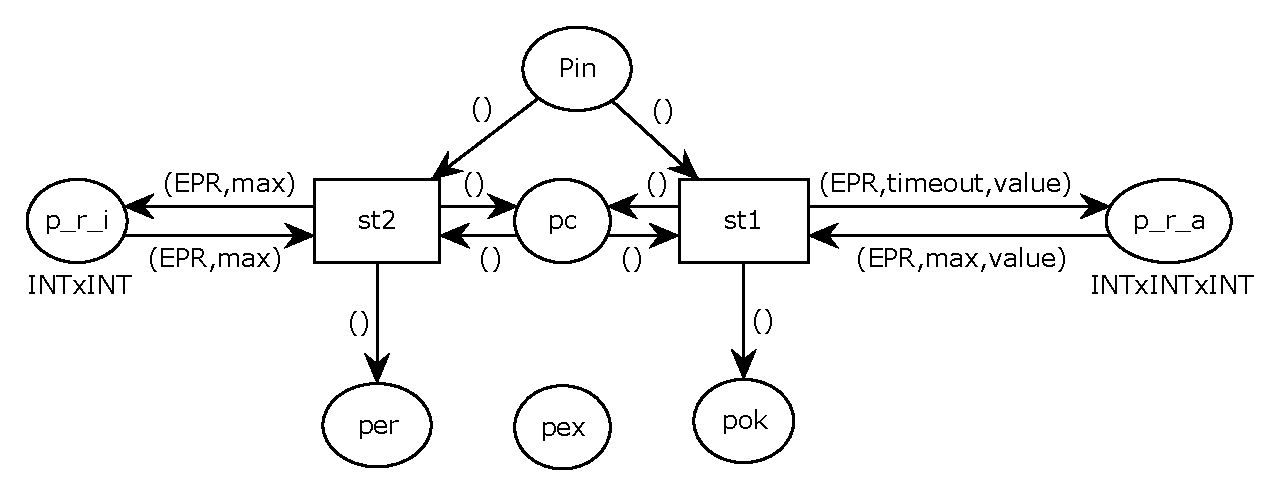
\includegraphics[scale=0.4]{Images/setTime.eps}}
%}}
%\end{center}
%\vspace{-0.62cm}
%\caption{\label{fig:sg}GetProperty and SetProperty Activities
%Translation}% \vspace{1cm}
%\vspace{-0.1cm}
%\end{figure}
%
%\newpage
\begin{figure}[!ht]
\begin{center}
\fbox{\parbox[t]{8.5cm}{\begin{center}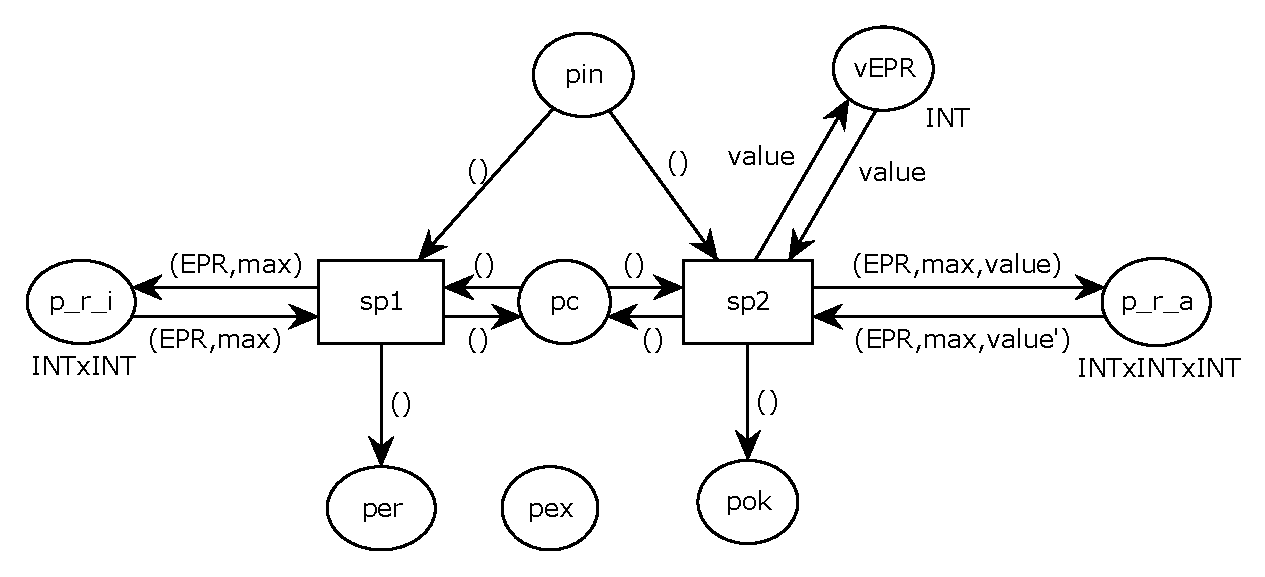
\includegraphics[scale=0.35]
{Images/setProp.eps}\end{center}}}
\end{center}
\vspace{-0.5cm}
\caption{\label{setp} SetProperty Activity Translation.}
%\vspace{0.5cm}
\end{figure}

\item {\it SetLifeTime(EPR,timeout)}:
This activity is analogous to {\em SetProp} activity. In this case, the resource lifetime is updated with a new value. Fig.~\ref{setp} shows this translation. 
\begin{figure}[!ht]
\begin{center}
%\vspace{-0.5cm}
\fbox{\parbox[t]{8.5cm}{\begin{center}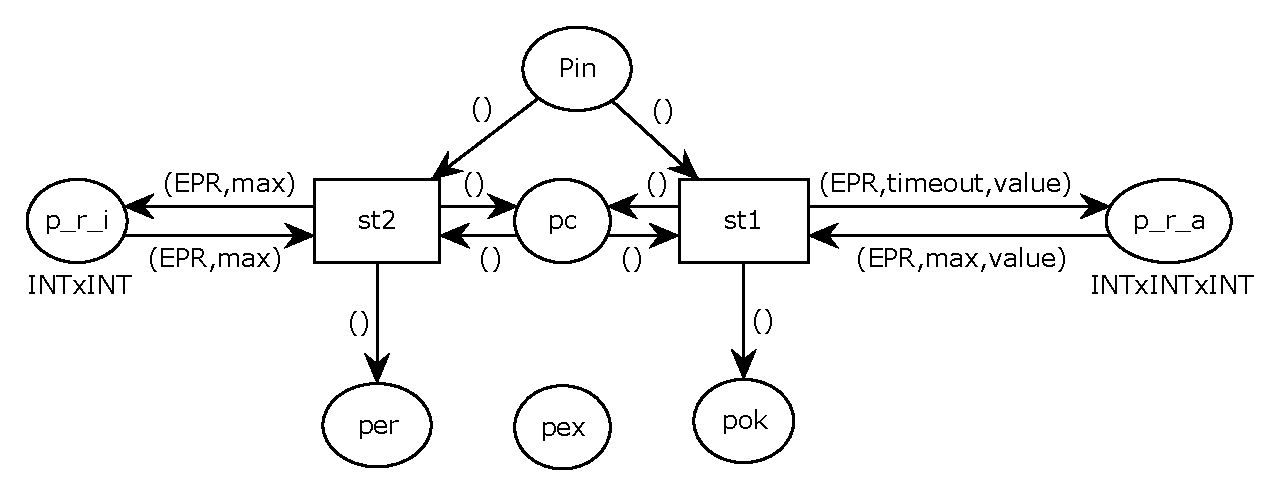
\includegraphics[scale=0.35]
{Images/setTime.eps}\end{center}}}
\end{center}
\vspace{-0.5cm}
\caption{\label{settim} SetLifeTime Activity Translation.}
%\vspace{-0.5cm}
\end{figure}
\end{itemize}

\subsection{Orchestration translation}
Once we have defined the translation for the activities, we can now introduce the definition
for the PTCPN at the orchestration level. Notice that all PTCPNs generated for
the different orchestrators cooperate to form  the entire system.

Let us call $N_A$, $N_{f}$ and $N_{e_i}$ the PTCPNs that
are obtained by applying the translation to each one of these
activities $A$, $A_f$, $A_{e_{i}},$ with $i\in\{1,m\}$:
%
\[
\begin{array}{lll}
N_A = (P_a, T_a, A_a, V_a, G_a, E_a, \lambda_a, D_a) &
\hspace*{0.6cm} & {\rm
(PTCPN~for~}A)\\
N_f = (P_f, T_f, A_f, V_f, G_f, E_f, \lambda_f, D_f)  &
\ & {\rm (PTCPN~for~}A_f)\\
N_{e_i} = (P_{e_i}, T_{e_i}, A_{e_i}, V_{e_i}, G_{e_i}, 
E_{e_i}, \lambda_{e_i}, D_{e_i})  &
\ & {\rm (PTCPN~for~}A_{e_i}\,)
\end{array}
\]

Let $p_{a_{\it in}}$, $p_{f_{\it in}}$ and $p_{{e_i}_{\it in}}$ be the initial places of
$N_A$, $N_f$ and $N_{e_i}$respectively; $p_{a_{\it ok}}$, $p_{f_{\it ok}}$ and $p_{{e_i}_{\it ok}}$ their {\em correct}\, output places, $p_{a_{\it er}},\, p_{f_{\it
er}}$ and $p_{{e_i}_{\it er}}$ their {\em error}\, places and, finally, $p_{a_{\it ex}},\, p_{f_{\it ex}}$ and $p_{{e_i}_{\it ex}}$ their {\em exit}\, places. The PTCPN for the
orchestrator is then constructed as indicated in Fig. \ref{orchestator}. This PTCPN is then activated by putting one token
$0$ on $p_{a_{\it in}}$. However, we can have other marked places, 
for instance, those associated with integer
variables or resources. The other places are initially unmarked.
%where we are joining the following places:
%
%\[\begin{array}{ l l l}
%p_{o_{\it in}} & = & p_{a_{\it in}} =  p_{{e_i}_{\it in}}\\
%
%p_{o_{\it er}} & = & p_{f_{\it ok}} = p_{f_{\it er}}\\
%
%p_{o_{\it ok}} & = & p_{a_{\it ok}} = p_{{e_i}_{\it ok}}\\
%
%p_{a_{\it er}} & = & p_{f_{\it in}}  =  p_{{e_i}_{\it er}}
%\end{array}
%\]
%
%and the remaining places, transitions and edges are the same as
%in $N_a$, $N_f$ and $N_{e_i}$.
% Marcado inicial:
%The PTCPN is then activated by putting one token
%$0$ on $p_{o_{\it in}}$. 
%
%
%as we mentioned when we introduced the PPTCPNs. 
%The other places are initially unmarked.

\begin{figure}[!ht]
%\vspace{-0.5cm}
\begin{center}
\fbox{ \parbox[t]{8cm}{ \center 
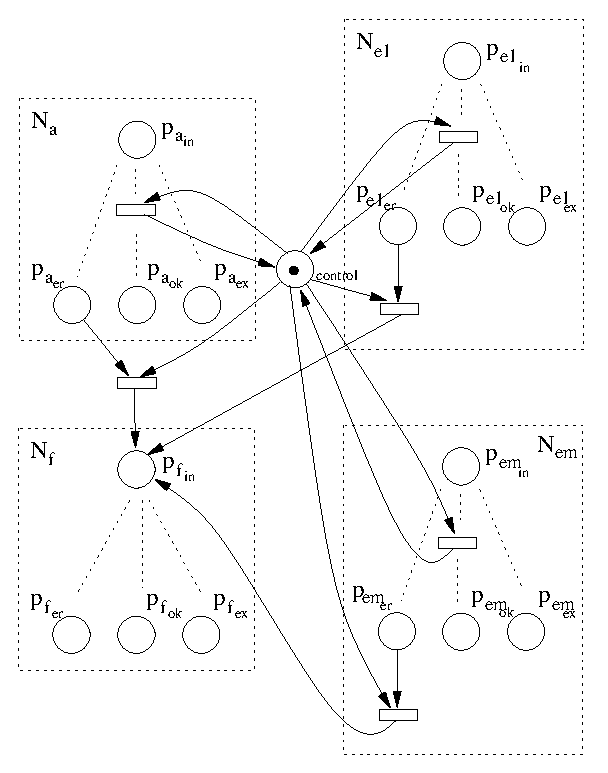
\includegraphics[scale=0.5]{Images/orchestration.eps}
}}\end{center}
\vspace{-0.5cm}
\caption{Orchestration Translation}\label{orchestator}
%\vspace{-0.5cm}
\end{figure}



